%%%%%%%%%%%%%%%%%%%%%%%%%%%%%%%%%%%%%%%%%%%%%%%%%%
%% Bachelor's & Master's Thesis Template        %%
%% Copyleft by Dawid Weiss & Marta Szachniuk    %%
%% Faculty of Computing and Telecommunication   %%
%% Poznan University of Technology, 2020        %%
%%%%%%%%%%%%%%%%%%%%%%%%%%%%%%%%%%%%%%%%%%%%%%%%%%


% Szkielet dla pracy licencjackiej pisanej w języku polskim.

\documentclass[polish,bachelor,a4paper,oneside]{ppfcmthesis}


\usepackage[utf8]{inputenc}
\usepackage[T1]{fontenc}
\usepackage{polski}
\usepackage{soul}
\usepackage{float}
\usepackage{hyphenat}
\usepackage{amssymb}
\usepackage{graphicx}
\usepackage{amsmath}
\usepackage{hyperref}
\usepackage{enumitem}
\usepackage{listingsutf8}
\usepackage{tcolorbox}
\usepackage{fancyvrb}
\usepackage{xcolor}

\definecolor{lightgray}{rgb}{0.95, 0.95, 0.95}
\definecolor{darkgray}{rgb}{0.4, 0.4, 0.4}
\definecolor{bglight}{gray}{0.95}

% Configure the listing style
\lstset{
    backgroundcolor=\color{bglight},
    basicstyle=\ttfamily\small,
    breaklines=true, 
    postbreak=\mbox{\textcolor{gray}{$\hookrightarrow$}\space},
    frame=single,
    rulecolor=\color{gray!30},
    captionpos=b,
    abovecaptionskip=10pt,
    extendedchars=true,
    literate={ą}{{\k{a}}}1 {ć}{{\'c}}1 {ę}{{\k{e}}}1 {ł}{{\l{}}}1 {ń}{{\'n}}1 {ó}{{\'o}}1 {ś}{{\'s}}1 {ź}{{\'z}}1 {ż}{{\.z}}1
             {Ą}{{\k{A}}}1 {Ć}{{\'C}}1 {Ę}{{\k{E}}}1 {Ł}{{\L{}}}1 {Ń}{{\'N}}1 {Ó}{{\'O}}1 {Ś}{{\'S}}1 {Ź}{{\'Z}}1 {Ż}{{\.Z}}1
}
\renewcommand{\lstlistingname}{WYKAZ}

\DeclareMathOperator*{\argmax}{argmax}

%--------------------------------------
% Strona tytułowa
%--------------------------------------

% Autorzy pracy, jeśli jest ich więcej niż jeden
% wstaw między nimi separator \and
\author{%
   Jakub Buler \album{155987} \and
   Adam Detmer \album{155976} \and 
   Jakub Kamieniarz \album{155845} \and
   Tomasz Pawłowski \album{155965}}
\authortitle{}                                % Do not change.

\title{Przetwarzanie języka naturalnego w celu sterowania aplikacją webową Moje Konie}

% Your supervisor comes here.
\ppsupervisor{dr inż.~Jędrzej Potoniec} 

% Year of final submission (not graduation!)
\ppyear{2026}                                 

\setcounter{tocdepth}{1} %  usuwa \subsection ze spisu treści.
\begin{document}

% Front matter starts here
\frontmatter\pagestyle{empty}%
\maketitle\cleardoublepage%

%--------------------------------------
% Miejsce na kartę pracy dyplomowej
%--------------------------------------

% \thispagestyle{empty}\vspace*{\fill}%
% \begin{center}Tutaj będzie karta pracy dyplomowej;\\oryginał wstawiamy do wersji dla archiwum PP, w pozostałych kopiach wstawiamy ksero.\end{center}%
% \vfill\cleardoublepage%

%--------------------------------------
% Spis treści
%--------------------------------------

\pagenumbering{Roman}\pagestyle{ppfcmthesis}%
\tableofcontents* 
\cleardoublepage % Zaczynamy od nieparzystej strony

%--------------------------------------
% Rozdziały
%--------------------------------------

%Najwygodniej jeśli każdy rozdział znajduje się w oddzielnym pliku
\mainmatter%
\input{chapters/01-wstep.tex}
\chapter{Przetwarzanie języka naturalnego i klasyfikacja intencji}
	
	\section{Wprowadzenie do przetwarzania języka naturalnego}

	\definicja{Przetwarzanie języka naturalnego} (\akronim{NLP}, \english{Natural Language Processing}) jest dziedziną sztucznej inteligencji, której celem jest umożliwienie komputerom zrozumienia, analizy i generowania ludzkiego języka w sposób, który jest zarówno wartościowy, jak i funkcjonalny \cite{aggarwal2018textbook}. \akronim{NLP} obejmuje szereg technik i metod, które pozwalają na wydobywanie znaczenia z tekstu w języku naturalnym, co jest kluczowe w systemach takich jak chatboty, wyszukiwarki internetowe czy asystenci głosowi.
	
	Z punktu widzenia technologii, NLP jest ściśle powiązane z takimi dziedzinami jak lingwistyka komputerowa, uczenie maszynowe, analiza tekstu i statystyka. W ciągu ostatnich kilku lat, dzięki postępom w głębokich sieciach neuronowych i modelach językowych, NLP osiągnęło ogromny postęp, umożliwiając bardziej precyzyjne rozumienie i generowanie tekstu.
	
	Jednym z najważniejszych osiągnięć w dziedzinie NLP jest koncepcja \definicja{osadzenia słów} (\english{word embeddings}), które stanowią matematyczne reprezentacje słów w przestrzeni wektorowej. Celem osadzenia słów jest odwzorowanie słów w przestrzeni, w której słowa o~podobnym znaczeniu mają podobne reprezentacje numeryczne, czyli znajdują się blisko siebie w tej przestrzeni.
	
	Do najbardziej popularnych algorytmów tworzenia osadzeń słów należą modele \definicja{Word2Vec} \cite{aggarwal2018textbook}, \definicja{GloVe} \cite{pennington2014glove} oraz nowsze podejścia oparte na transformatorach, takie jak \definicja{BERT} \cite{devlin2018bert} czy \definicja{GPT} \cite{radford2019gpt2}. W tych modelach każde słowo w tekście jest reprezentowane przez wektor liczb, który odzwierciedla jego semantykę oraz kontekst użycia. Modele te bazują na analizie kontekstów słów w dużych korpusach tekstów, co pozwala na wyłapywanie zależności pomiędzy słowami.
	
	Szczególnie istotnym rozszerzeniem jest \definicja{Sentence-BERT (SBERT)}, umożliwiający tworzenie wektorów reprezentujących całe zdania, co czyni go niezwykle użytecznym w klasyfikacji tekstu, wyszukiwaniu informacji czy dopasowaniu zapytań \cite{reimers2019sentencebert}.

	\section{Klasyfikatory intencji}
	% TODO: odpowiedniej czego
	Klasyfikator intencji jest mechanizmem, który ma na celu przypisanie zapytania użytkownika do odpowiedniej końcówki \cite{aggarwal2018textbook}. W kontekście NLP klasyfikatory intencji najczęściej wykorzystują osadzenia słów oraz różne techniki dopasowania, takie jak podobieństwo kosinusowe, do porównania zapytań z wcześniej zdefiniowanymi przykładami. Celem tych systemów jest przypisanie odpowiedniego kontekstu do zapytania, co pozwala na efektywne sterowanie aplikacjami lub systemami, jak np. asystenci głosowi, chatboty czy systemy rekomendacji.
	
	\definicja{Intencje użytkowników} są zazwyczaj definiowane poprzez zestaw fraz, które mogą być używane przez użytkownika do wyrażenia swojej woli. Każda fraza przypisana jest do określonej intencji, a klasyfikator intencji jest odpowiedzialny za przypisanie zapytania użytkownika do jednej z tych intencji.
	
	Klasyfikacja intencji jest realizowana przez modele oparte na głębokich sieciach neuronowych, które są trenowane na dużych zbiorach danych. Modele te uczą się rozpoznawania wzorców w tekstach, dzięki czemu mogą efektywnie klasyfikować zapytania do odpowiednich kategorii. Wykorzystanie technik takich jak osadzenia słów oraz podobieństwo kosinusowe pozwala na efektywne porównanie zapytań użytkowników z wcześniej zdefiniowanymi intencjami, co pozwala na przypisanie odpowiednich akcji lub odpowiedzi w systemach bazujących na NLP.

	Po utworzeniu osadzenia słów, kolejnym krokiem w NLP jest ocena podobieństwa między różnymi wektorami. Najczęściej używaną miarą w tym przypadku jest podobieństwo kosinusowe (\english{cosine similarity}), które mierzy kąt między dwoma wektorami w przestrzeni wektorowej. Miara ta jest szczególnie użyteczna, ponieważ daje wynik w zakresie od -1 do 1, gdzie wartość 1 oznacza wektory identyczne, wartość -1 oznacza wektory całkowicie przeciwne.

	Matematyczna ocena pokrewieństwa semantycznego między zapytaniem a bazą wzorców opiera się na analizie geometrii wektorów, a nie na bezpośrednim dopasowywaniu znaków. Kluczowym narzędziem wykorzystywanym w tym procesie jest podobieństwo kosinusowe, które mierzy cosinus kąta między dwoma wektorami w przestrzeni 1024-wymiarowej. Wybór tej metryki, opisanej wzorem (\ref{eq:cosine}), wynika z jej odporności na różnice w długości tekstów; w systemach NLP istotny jest kierunek wektora, reprezentujący temat wypowiedzi, a nie jego norma (długość), która często zależy jedynie od liczby użytych słów.

	\begin{equation}
		\text{similarity}(A, B) = \cos(\theta) = \frac{A \cdot B}{\|A\| \|B\|} = \frac{\sum_{i=1}^{n} A_i B_i}{\sqrt{\sum_{i=1}^{n} A_i^2} \sqrt{\sum_{i=1}^{n} B_i^2}} 
		\label{eq:cosine}
	\end{equation}

	Wartość tej miary oscyluje w granicach od -1 do 1, gdzie 1 oznacza identyczność semantyczną. Dzięki temu system jest w stanie poprawnie zakwalifikować zapytania takie jak ,,Dodaj wizytę kowala'' oraz ,,Kowal był u konia'', mimo że na poziomie leksykalnym dzielą one jedynie jedno słowo kluczowe \cite{han2011}.

	W kontekście klasyfikacji intencji, podobieństwo kosinusowe pozwala na ocenę, jak blisko w~przestrzeni wektorowej znajdują się zapytania użytkowników względem dostępnych przykładów \cite{aggarwal2018textbook}. Dzięki temu możliwe jest przypisanie odpowiednich końcówek \termdef{Application Programming Interface} (\akronim{API}) do zapytań użytkowników w systemach sterowanych językiem naturalnym.

	Współczesne podejścia coraz częściej wykorzystują modele oparte na transformatorach, które umożliwiają rozpoznawanie intencji nawet w kontekście nieznanych wcześniej sformułowań (\definicja{few-shot} lub \definicja{zero-shot learning}) \cite{brown2020language}. Takie podejście sprawia, że systemy NLP są znacznie bardziej elastyczne i odporne na wariacje językowe użytkowników.
	
	\section{Transformatory i mechanizm uwagi}
	
	Transformatory to jedna z najnowszych i najbardziej przełomowych architektur w dziedzinie NLP, wprowadzona przez Vaswaniego i współpracowników w \cite{vaswani2017attention}. Głównym celem tej architektury było poprawienie efektywności modeli językowych poprzez wyeliminowanie rekurencyjnych warstw, które były wykorzystywane w poprzednich modelach, takich jak LSTM \cite{hochreiter1997lstm} i GRU \cite{cho2014gru}. Transformator jest oparty na mechanizmie samo-uwagi (\english{self-attention}), który umożliwia modelowi analizowanie wszystkich słów w zdaniu równocześnie i decydowanie o tym, które słowa są najbardziej istotne w kontekście innych słów.
	
	Mechanizm uwagi (\english{attention mechanism}) jest kluczowym elementem działania transformatora i służy do ważenia różnych słów w zdaniu na podstawie ich istotności. Działa to w następujący sposób: dla każdego słowa w zdaniu model przypisuje wagę, która zależy od tego, jak ważne jest to słowo w kontekście innych słów w zdaniu. Dzięki temu, model może uwzględnić nie tylko lokalne zależności między słowami, ale także globalne konteksty, co znacznie poprawia jakość przetwarzania informacji.
	
	W mechanizmie uwagi transformatora każdy token, czyli jednostka tekstu, na jaką model językowy dzieli dane wejściowe, jest reprezentowany przez trzy wektory: zapytanie (\english{query}), klucz (\english{key}) oraz wartość (\english{value}). Wagi uwagi oblicza się na podstawie iloczynu skalarnego zapytania i klucza, a następnie stosuje się funkcję \textit{softmax}, aby uzyskać rozkład prawdopodobieństwa nad wszystkimi słowami. Na przykład, w zdaniu:  \textit{„Właściciel konia chce dodać nową klacz do hodowli”},  token \textit{„właściciel”} może otrzymać wysoką wagę względem słów \textit{„chce”} i \textit{„klacz”}, ponieważ to one definiują działanie użytkownika.
	
	Największą zaletą transformatorów w porównaniu do wcześniejszych modeli rekurencyjnych, takich jak LSTM\cite{hochreiter1997lstm} czy GRU\cite{cho2014gru}, jest ich zdolność do równoczesnego przetwarzania wszystkich słów w zdaniu (równoległość), co znacznie przyspiesza proces trenowania. Ponadto, dzięki mechanizmowi uwagi, modele transformatorów są w stanie uchwycić długoterminowe zależności w tekście, co jest trudne do osiągnięcia w modelach sekwencyjnych.
	
	Transformatory stały się podstawą dla wielu dużych modeli językowych: \definicja{BERT} \cite{devlin2018bert}, \definicja{GPT-2} \cite{radford2019gpt2}, \definicja{GPT-3} \cite{brown2020language}, które osiągnęły znaczące sukcesy w zadaniach NLP, takich jak klasyfikacja tekstów \cite{devlin2018bert}, tłumaczenie maszynowe \cite{vaswani2017attention}, generowanie tekstu \cite{brown2020language}, odpowiedzi na pytania \cite{devlin2018bert} czy analiza sentymentu \cite{devlin2018bert}.

    Ostatni etap rozwoju NLP to pojawienie się \definicja{dużych modeli językowych} (\akronim{LLM}, \english{Large Language Models}), które wykorzystują miliardy parametrów do modelowania języka na podstawie ogromnych korpusów danych. Modele te, oparte na architekturze transformatora, potrafią wykonywać złożone zadania, takie jak tłumaczenie, streszczanie, generowanie kodu czy prowadzenie rozmowy \cite{openai2023gpt4technicalreport}.
    
    Jednym z najnowszych osiągnięć jest seria modeli \definicja{Gemini}, opracowana przez Google DeepMind. \definicja{Gemini 2.5 Flash}, łączy multimodalność (obsługuje tekst, obraz, dźwięk i wideo) z długim kontekstem przekraczającym milion tokenów. Model ten posiada zdolność wnioskowania -- tzn. rozwiązywania problemów poprzez wieloetapowe rozumowanie i planowanie działań, co określane jest mianem „\definicja{thinking model}” \cite{deepmind2025gemini}.  
    Dzięki integracji z narzędziami (\definicja{tool use} / \definicja{function calling}), Gemini 2.5 Flash może wykonywać rzeczywiste operacje -- np. wywoływać API, generować zapytania REST czy wykonywać obliczenia. W kontekście niniejszej pracy model ten może zatem nie tylko klasyfikować intencje użytkowników, ale także automatycznie generować odpowiednie żądania HTTP, umożliwiając naturalne sterowanie aplikacją webową.  
    Mimo wysokiej skuteczności, LLM-y takie jak Gemini 2.5 Flash nadal wymagają dużych zasobów obliczeniowych i mogą generować nieścisłości semantyczne, znane jako \definicja{halucynacje} \cite{bommasani2021opportunities}.

	\section{Podsumowanie}
	
	Przetwarzanie języka naturalnego stanowi jeden z fundamentów współczesnych systemów inteligentnych, umożliwiając komputerom interakcję z użytkownikami w sposób zbliżony do ludzkiego. Modele osadzania słów, takie jak Word2Vec, GloVe, BERT czy Sentence-BERT, stanowią podstawę nowoczesnych rozwiązań NLP, pozwalając na analizę i klasyfikację tekstów. Dopasowanie kosinusowe jest jedną z najczęściej stosowanych miar podobieństwa, umożliwiającą efektywne porównywanie zapytań użytkowników z przykładami intencji w systemach klasyfikacji. Klasyfikatory intencji, oparte na tych technologiach, umożliwiają skuteczne przypisanie zapytań do odpowiednich działań w aplikacjach, takich jak chatboty czy asystenci głosowi.
	
	Współczesne modele oparte na mechanizmie uwagi, takie jak transformatory, zrewolucjonizowały dziedzinę NLP, oferując wydajność i dokładność, które były niemożliwe do osiągnięcia w poprzednich modelach. Dzięki transformatorom możliwe stało się przetwarzanie długich tekstów oraz uchwycenie głębokich, globalnych zależności w tekście.
	Od prostych modeli osadzania słów, przez transformery, aż po duże modele językowe -- rozwój NLP umożliwia coraz bardziej naturalną interakcję człowieka z komputerem. Zastosowanie LLM, takich jak \definicja{Gemini 2.5 Flash}, otwiera nowe możliwości dla aplikacji sterowanych językiem naturalnym, w tym systemu \definicja{Moje Konie}, w którym polecenia użytkownika mogą być tłumaczone bezpośrednio na żądania REST w sposób kontekstowo poprawny i semantycznie spójny.
	

\input{chapters/03-architektura.tex}
\input{chapters/04-front.tex}
\chapter{Opracowanie i~ocena eksperymentalna klasyfikatora intencji użytkownika} \label{sec:klasyfikator}
\label{chapters:05-Klasyfikator_intencji}

\section{Wyzwania interpretacji semantycznej poleceń użytkownika}

Głównym celem projektowanego modułu \definicja{Asystenta NLP} w systemie \definicja{Moje Konie} jest umożliwienie użytkownikowi, najczęściej hodowcy koni lub pracownikowi stajni, interakcji z systemem za pomocą języka naturalnego. 

Jak wskazuje w swoich pracach Christopher Manning \cite{manning2008}, współczesne wyzwanie w przetwarzaniu języka naturalnego (NLP) przesunęło się z prostego rozpoznawania słów w stronę głębokiego rozumienia intencji i kontekstu, co jest kluczowe dla budowy systemów zdolnych do realnej pomocy człowiekowi w konkretnych dziedzinach życia.

W specyficznych warunkach pracy terenowej, takich jak stajnia czy padok, tradycyjne wprowadzanie danych poprzez formularze webowe jest często niepraktyczne. Rozwiązaniem jest interfejs konwersacyjny (czat lub komendy głosowe), który przekłada swobodną wypowiedź na ustrukturyzowane żądanie do bazy danych. Zadanie to wymaga od systemu nie tylko rozpoznania fonetycznego lub tekstowego, ale przede wszystkim precyzyjnego przypisania wypowiedzi do odpowiedniej akcji w systemie (\english{Intent Classification}).

\subsection*{Definicja problemu mapowania intencji}

System musi być zdolny do poprawnej interpretacji i przekierowania zapytania do jednego z~ośmiu predefiniowanych obszarów funkcjonalnych (końcówek REST API), obsługujących zarządzanie hodowlą:
\begin{description}
    \item[Zarządzanie stadem:] rejestracja i edycja koni (\texttt{/api/konie}).
    \item[Rozród:] ewidencja kryć, wyźrebień i kontroli weterynaryjnej rozrodu (\texttt{/api/wydarzenia/rozrody}).
    \item[Profilaktyka:] odnotowywanie szczepień, odrobaczania, suplementacji czy wizyt dentystycznych (\texttt{/api/wydarzenia/zdarzenia\_profilaktyczne}).
    \item[Pielęgnacja kopyt:] dokumentowanie wizyt kowala i zabiegów werkowania (\texttt{/api/wydarzenia/\allowbreak{}podkucie}).
    \item[Weterynaria i zdrowie:] monitorowanie procesów leczenia (\texttt{/api/wydarzenia/leczenia}), diagnozowanie chorób (\texttt{/api/wydarzenia/choroby})
    \item[Baza kontaktów:] zarządzanie bazą kontaktów do specjalistów (\texttt{/api/kowale}, \texttt{/api/weterynarze}).
\end{description}

\subsection*{Trudności w przetwarzaniu języka naturalnego (NLP)}

Zrozumienie intencji użytkownika w tym konkretnym przypadku napotyka na bariery, które w~literaturze przedmiotu uznaje się za kluczowe problemy NLU (\textit{Natural Language Understanding})~\cite{jurafsky2023}:

\begin{description}
    \item[Zróżnicowanie lingwistyczne i semantyczne:] Użytkownicy używają różnych konstrukcji dla tej samej czynności (np. ,,Kasztanka została zaszczepiona'' vs ,,Dodaj szczepienie dla Kasztanki''). Zgodnie z tezą Manninga \cite{manning2008}, system musi tu wykazać się zdolnością rozumienia, by odwzorować oba sformułowania na właściwą końcówkę profilaktyki.
    
    \item[Specjalistyczna terminologia:] Branża jeździecka operuje słownictwem (np. ,,werkowanie'', ,,źrebność''), które rzadko występuje w korpusach języka ogólnego, co wymaga od modelu wysokiej jakości reprezentacji wektorowych (\english{embeddings}) zdolnych do uchwycenia relacji między tymi terminami a ich medycznym znaczeniem.
\end{description}

\section{Ewolucja architektury: od modelu monolitycznego do podejścia hybrydowego}

W początkowej fazie projektowania systemu asystenta, proces interpretacji zapytania opierał się na architekturze monolitycznej z wykorzystaniem dużych modeli językowych (LLM). W tym podejściu surowy tekst użytkownika był przesyłany bezpośrednio do modelu (np. Gemini lub DeepSeek) wraz z pełną dokumentacją wszystkich ośmiu dostępnych punktów końcowych API w~jednym zapytaniu. Zadaniem modelu było jednoczesne rozpoznanie intencji oraz wygenerowanie poprawnie sformatowanego obiektu JSON, służącego jako ciało żądania HTTP.

\subsection{Ograniczenia podejścia monolitycznego}

Wstępne testy wykazały, że mimo wysokiej elastyczności modeli LLM, takie rozwiązanie posiada istotne wady z punktu widzenia wydajności systemu:

\begin{description}
	\item[Nadmiarowość kontekstu:] Dołączanie pełnego schematu API (wszystkich ośmiu końcówek) do każdego zapytania drastycznie zwiększało liczbę tokenów wejściowych. Generuje to nieuzasadnione koszty operacyjne, zwłaszcza przy częstym korzystaniu z płatnych API, oraz zwiększa czas oczekiwania na odpowiedź \cite{liu2023}, a~zatem takie rozwiązanie nie jest skalowane do większych systemów.
    
	\item[Szum informacyjny:] Przekazywanie do modelu informacji o końcówkach niezwiązanych z danym zapytaniem (np. schemat rozrodu przy pytaniu o kowala) zwiększa ryzyko halucynacji. Model, mając zbyt szeroki kontekst, może próbować odwzorowywać dane do niewłaściwych pól, co obniża ogólną precyzję żądania.
    
	\item[Trudność w debugowaniu:] Przy podejściu ,,wszystko w jednym'', trudno jest jednoznacznie określić, czy błąd wynika z błędnego rozpoznania intencji, czy z problemów modelu ze zbudowaniem poprawnego obiektu JSON.
\end{description}

\subsection{Przejście na model hybrydowy}

Zdecydowano się na zmianę architektury na model hybrydowy, w którym proces przetwarzania zapytania został rozdzielony na dwa etapy. Pierwszym krokiem jest wykorzystanie dedykowanego, ,,lekkiego'' klasyfikatora opartego na osadzeniach wektorowych (\english{word/sentence embeddings}), którego jedynym zadaniem jest identyfikacja intencji użytkownika.
Głównym założeniem tej zmiany było przeniesienie ciężaru klasyfikacji na lokalny lub tańszy w~eksploatacji model wektorowy, co pozwoliło na:

\begin{description}
	\item[Dynamiczne budowanie zapytania:] Do modelu LLM wysyłany jest wyłącznie ten fragment dokumentacji API, który jest bezpośrednio związany z intencją wykrytą przez klasyfikator. Takie podejście, znane jako \textit{context pruning}, pozwala na redukcję rozmiaru zapytania o~znaczący procent, co przekłada się na realne oszczędności tokenów \cite{jimenez2022}.
    
	\item[Większą precyzję odwzorowania:] Model LLM, otrzymując instrukcję dotyczącą tylko jednej, konkretnej końcówki, rzadziej popełnia błędy w~odwzorowaniu pól technicznych i lepiej radzi sobie z ekstrakcją parametrów z tekstu.
    
	\item[Separację logiki:] Wyodrębnienie klasyfikatora pozwoliło na precyzyjne dostrajanie procesu wykrywania intencji (np. poprzez wykorzystanie algorytmu k-NN i doborze jego hiperparemetrów) niezależnie od warstwy generatywnej.
\end{description}

Wdrożenie tej separacji umożliwiło nam zbadanie, jak klasyczne metody uczenia maszynowego operujące na wektorach semantycznych radzą sobie z branżowym słownictwem.
Nasz problem jednak wciąż wiązał się z:

\begin{description}
    \item[Niejasnością i skrótowością:] Krótkie komunikaty wysyłane w pośpiechu (np. ,,kowal u Gwiazdy'') wymuszają na systemie automatyczne rozpoznanie, że chodzi o wizytę kowala i przypisanie jej do konkretnego konia, co bez zrozumienia kontekstu branżowego byłoby niemożliwe.
    \item[Ekstrakcją encji:] Poza samą intencją, system musi ,,wyłowić'' z tekstu kluczowe parametry (np. imię konia, datę, nazwę leku), by stworzyć poprawne żądanie POST do API.
\end{description}

W związku z powyższym, proste dopasowanie słów kluczowych okazało się niewystarczające. Zdecydowaliśmy się stworzyć architekturę, która połączy elastyczność dużych modeli językowych (LLM) z precyzją i wydajnością klasyfikatorów wektorowych. Klasyfikator wektorowy został przeznaczony do rozwiązania problemu klasyfikacji intencji, a na LLM została zrzucona cała odpowiedzialność wypełnienia żądania mając już informacje o końcówce.

\section{Metodyka i implementacja klasyfikatora intencji}

Fundamentem działania nowoczesnych systemów rozumienia tekstu jest transformacja symboli językowych na gęste reprezentacje wektorowe w przestrzeni wielowymiarowej. W projektowanym systemie proces ten realizowany jest za pomocą zaawansowanego modelu osadzeń słów (\english{embeddings}) \texttt{multilingual-e5-large-instruct}, który opiera się na architekturze transformatora.

W przeciwieństwie do tradycyjnych metod, takich jak Bag-of-Words czy TF-IDF, które bazują na częstotliwości występowania słów, modele oparte na osadzeniach kodują relacje semantyczne i kontekstualne. Model E5 generuje wektory o stałej długości 1024 komponentów, co pozwala na uchwycenie subtelnych różnic znaczeniowych między zapytaniami.

Wykorzystanie wariantu ,,instruct'' wprowadza dodatkową warstwę precyzji -- system wymaga stosowania prefiksów instrukcyjnych (np. \texttt{query:} dla danych wejściowych użytkownika oraz \texttt{passage:} dla wzorców w bazie wiedzy). 
Taka asymetria w procesie wektoryzacji jest kluczowa dla efektywnego mapowania krótkich, często niekompletnych pytań na opisy funkcji systemowych zawarte w~dokumentacji API \cite{reimers2019}.

W praktycznej implementacji proces ten opiera się na dwóch niezależnych strumieniach danych, integrowanych w wspólnej przestrzeni wektorowej. Pierwszym z nich jest dynamiczne zapytanie użytkownika (\textit{query}), czyli surowa wypowiedź naturalna, która po procesie normalizacji jest zamieniana na wektor . Drugim elementem jest statyczna baza wiedzy, składająca się w bieżącej wersji systemu z 480 zdefiniowanych przykładów (\textit{passages}), reprezentujących wzorcowe sformułowania dla poszczególnych intencji.

Poniższy przykład ilustruje strukturę przygotowania danych przed ich wektoryzacją, prezentując transformację zapytania użytkownika o nowym koniu oraz fragment bazy 480 wzorców:

\begin{verbatim}
# 1. STRUMIEŃ ZAPYTANIA (Query) - wypowiedź użytkownika
"query: dodaj nowego konia blyskawica to 6 letnia klacz wlasnie ja przywiozlem"

# 2. STRUMIEŃ BAZY WIEDZY (Passages) - wybrane z 480 przykładów
"passage: chce dodac mloda klacz kore do hodowli"
"passage: prosze wprowadzic nowego konia brego kon rekreacyjny czteroletni"
"passage: dodaj do mojej stajni 6 letniego ogiera zenita"
"passage: dopisz konia neptuna mlodego walacha do jazdy terenowej"
"passage: zarejestruj w hodowli klacz melodie 3 lata"
\end{verbatim}



Zastosowana asymetria pozwala na obliczenie podobieństwa cosinusowego między wektorem zapytania a każdym z wektorów bazy. Dzięki semantycznemu kodowaniu modelu E5, system potrafi zidentyfikować, że potoczna fraza „właśnie ją przywiozłem” w połączeniu z opisem zwierzęcia odpowiada intencji rejestracji nowego obiektu, wykazując najwyższą korelację z przykładami takimi jak „wprowadź nowego konia” czy „dopisz konia do stajni”.



\subsection*{Baza wiedzy i kotwice}

Skuteczność klasyfikacji w systemach dedykowanych dziedzinowo jest nierozerwalnie związana z~jakością bazy wiedzy, która pełni rolę semantycznego układu odniesienia. W ramach implementacji przygotowano zestaw wzorcowych intencji, z których każda odpowiada jednej z ośmiu końcówek API. Każda intencja reprezentowana jest przez zestaw tzw. kotwic (\english{anchors}) -- starannie dobranych sformułowań, które modelują typowy sposób komunikacji użytkownika. Proces ten można przyrównać do nadzorowanego uczenia maszynowego typu \textit{few-shot learning}, gdzie system uczy się rozpoznawać kategorie na podstawie ograniczonej liczby przykładów.

Zastosowanie {dużych modeli językowych} (\akronim{LLM}) sprawia dodatkowo, że system wykazuje się wysoką odpornością na błędy gramatyczne oraz zapożyczenia, co w specyficznym języku hodowców koni, łączącym potoczne sformułowania z branżową terminologią specjalistyczną, ma fundamentalne znaczenie \cite{wang2022}.

\subsection*{Ewolucja algorytmu: od k-NN do centroidów}

W dążeniu do poprawy zdolności klasyfikatora do generalizacji, ewolucja algorytmu decyzyjnego zakładała przejście od analizy punktowej do modelowania uśrednionego rozkładu kategorii. Pierwotnie zaimplementowany algorytm K-Najbliższych Sąsiadów (k-NN) dla $k=1$ charakteryzował się dużą czułością na jednostkowe sformułowania wzorcowe.

Jako istotną poprawkę zaproponowano klasyfikację opartą na centroidach kategorii. W tym modelu każda z ośmiu intencji reprezentowana jest przez pojedynczy wektor centroidu $C_i$, obliczany jako średnia arytmetyczna wszystkich wektorów wzorcowych danej klasy, zgodnie ze wzorem (\ref{eq:centroid}).

\begin{equation}
    C_i = \frac{1}{N} \sum_{j=1}^{N} v_{i,j}
    \label{eq:centroid}
\end{equation}

\noindent gdzie:
\begin{itemize}
    \item $C_i$ -- wektor centroidu odpowiadający $i$-tej intencji,
    \item $v_{i,j}$ -- $j$-ty wektor wzorcowy należący do intencji $i$,
    \item $N$ -- liczba wektorów wzorcowych przypisanych do danej intencji.
\end{itemize}

Celem tej modyfikacji było wyznaczenie stabilnego „środka ciężkości” dla każdej operacji dostępnej w interfejsie API. W tak zdefiniowanej przestrzeni metrycznej, proces decyzyjny klasyfikatora polega na wyznaczeniu miary podobieństwa cosinusowego między wektorem zapytania użytkownika $q$ a wszystkimi centroidami $C_i$. Ostateczna klasyfikacja dokonywana jest poprzez wybór intencji, która wykazuje najwyższą wartość tego podobieństwa, co można zapisać za pomocą operatora argumentu maksymalizującego:

\begin{equation}
    \text{intent} = \arg\max_{i} \left( \frac{q \cdot C_i}{\|q\| \|C_i\|} \right)
\end{equation}

Podejście to pozwoliło na zredukowanie wpływu szumu informacyjnego oraz wyeliminowanie problemu nadmiernej czułości na odosobnione, nietypowe sformułowania znajdujące się w bazie wzorców. Dzięki uśrednieniu reprezentacji wektorowych, model zyskał wyższą zdolność do generalizacji, skupiając się na kluczowych cechach semantycznych wspólnych dla całej grupy 480 przykładów definiujących logiczne punkty końcowe systemu.

\subsection*{Logika decyzyjna i progi pewności}

Krytyczna analiza zachowania modelu pozwoliła na uproszczenie logiki decyzyjnej poprzez rezygnację z pierwotnie planowanych progów pewności (\english{confidence thresholds}), które zmuszały klasyfiakator do analizowania słów kluczowych. Doświadczenia wykazały jednak, że model osiąga skrajnie niskie wartości podobieństwa niemal wyłącznie w sytuacjach, gdy wprowadzony tekst jest zupełnie pozbawiony informacji semantycznych co przekłada się na niemożność zbudowania poprawnego zapytania w póżniejszym etapie. W sytuacjach, gdy użytkownik formułuje jakąkolwiek intencję związaną z domeną systemu, model z dużą precyzją wskazuje właściwy kierunek semantyczny.

\section{Benchmarking i optymalizacja}

\subsection{Dane użyte w eksperymencie}

W celu empirycznego wyznaczenia optymalnej konfiguracji dla systemu \definicja{Moje Konie}, przeprowadzono serię testów ewaluacyjnych. Do eksperymentu przyjęto zbiór danych podzielony na:
\begin{description}
	\item[Bazę wiedzy:] 60 reprezentatywnych przykładów, pełniących funkcję kotwic (\english{anchors}).
	\item[Zbiór testowy:] 40 unikalnych, nieznanych modelowi przykładów.
\end{description}

Dane były generowane ręcznie przez uczestników projektu, którzy na podstawie swojego doświadczenia z hodowcami koni próbowali odtworzyć ich sposób mówienia, jednocześnie zapewniając, że przykłady spełniają podstawowe wymagania systemu. Zależało nam, że nasz zbiór danych pokrywał różny poziom formalności przekazywanai informacji stąd np. w końcówce \texttt{api/wydarzenia/\allowbreak{}rozrody} znajdują się przykłady takie jak:

\begin{itemize}
    \item ,,Dino miał dzisiaj sprawdzanie źrebności. Alicja powiedziała, że wszystko było ok'',
    \item ,,Dodaj proszę informację, że klacz Bella była dziś inseminowana przez dr Kowalską'',
    \item ,,Wczoraj Tomek podkuł Lasera''.
\end{itemize}
Dane zostały przygotowane w formacie JSON, gdzie dla każdej końcówki przypisana jest lista zdań.

\subsection{Metodyka benchmarkingu hiperparametru sąsiedztwa}

Kluczowym aspektem strojenia modelu opartego na algorytmie k-NN  jest dobór odpowiedniej wielkości sąsiedztwa $k$, która determinuje strefę wpływu lokalnego na decyzję klasyfikacyjną \cite{manning2008}.
Ewaluację przeprowadzono dla zmiennych wartości $k$, mierząc skuteczność za pomocą metryk: dokładność (\english{accuracy}) oraz F1-makro. Wybór F1-makro był podyktowany koniecznością równoprawnego traktowania wszystkich intencji.

\subsection*{Strategia rozstrzygania remisów}

W klasycznym algorytmie k-NN dochodzi do sytuacji spornych, gdzie dwie lub więcej klas otrzymują identyczną liczbę głosów. W badanej implementacji zastosowano heurystykę opartą na gęstości semantycznej. W przypadku remisu głosów, ostateczna predykcja $y_{pred}$ jest wybierana na podstawie sumy podobieństw cosinusowych sąsiadów należących do danej klasy:

\begin{equation}
    y_{pred} = \argmax_{c \in C_{tied}} \left( \sum_{i \in N_c} \cos(\vec{x}, \vec{x}_i) \right)
\end{equation}
%
gdzie $N_c$ to zbiór sąsiadów należących do spornej klasy $c$, a $\vec{x}$ to wektor zapytania. Takie podejście premiuje klasę, której przykłady znajdują się ,,semantycznie bliżej'' zapytania użytkownika.
W~ramach eksperymentu przeprowadzono ewaluację algorytmu k-NN dla wartości parametru $k$~w~zakresie od 1 do 20 dla pełnego zbioru danych. Wyniki uzyskane dla zbioru testowego przedstawiono na Rysunku~\ref{fig:knn_eval}.

\begin{figure}%[H]
    \centering
    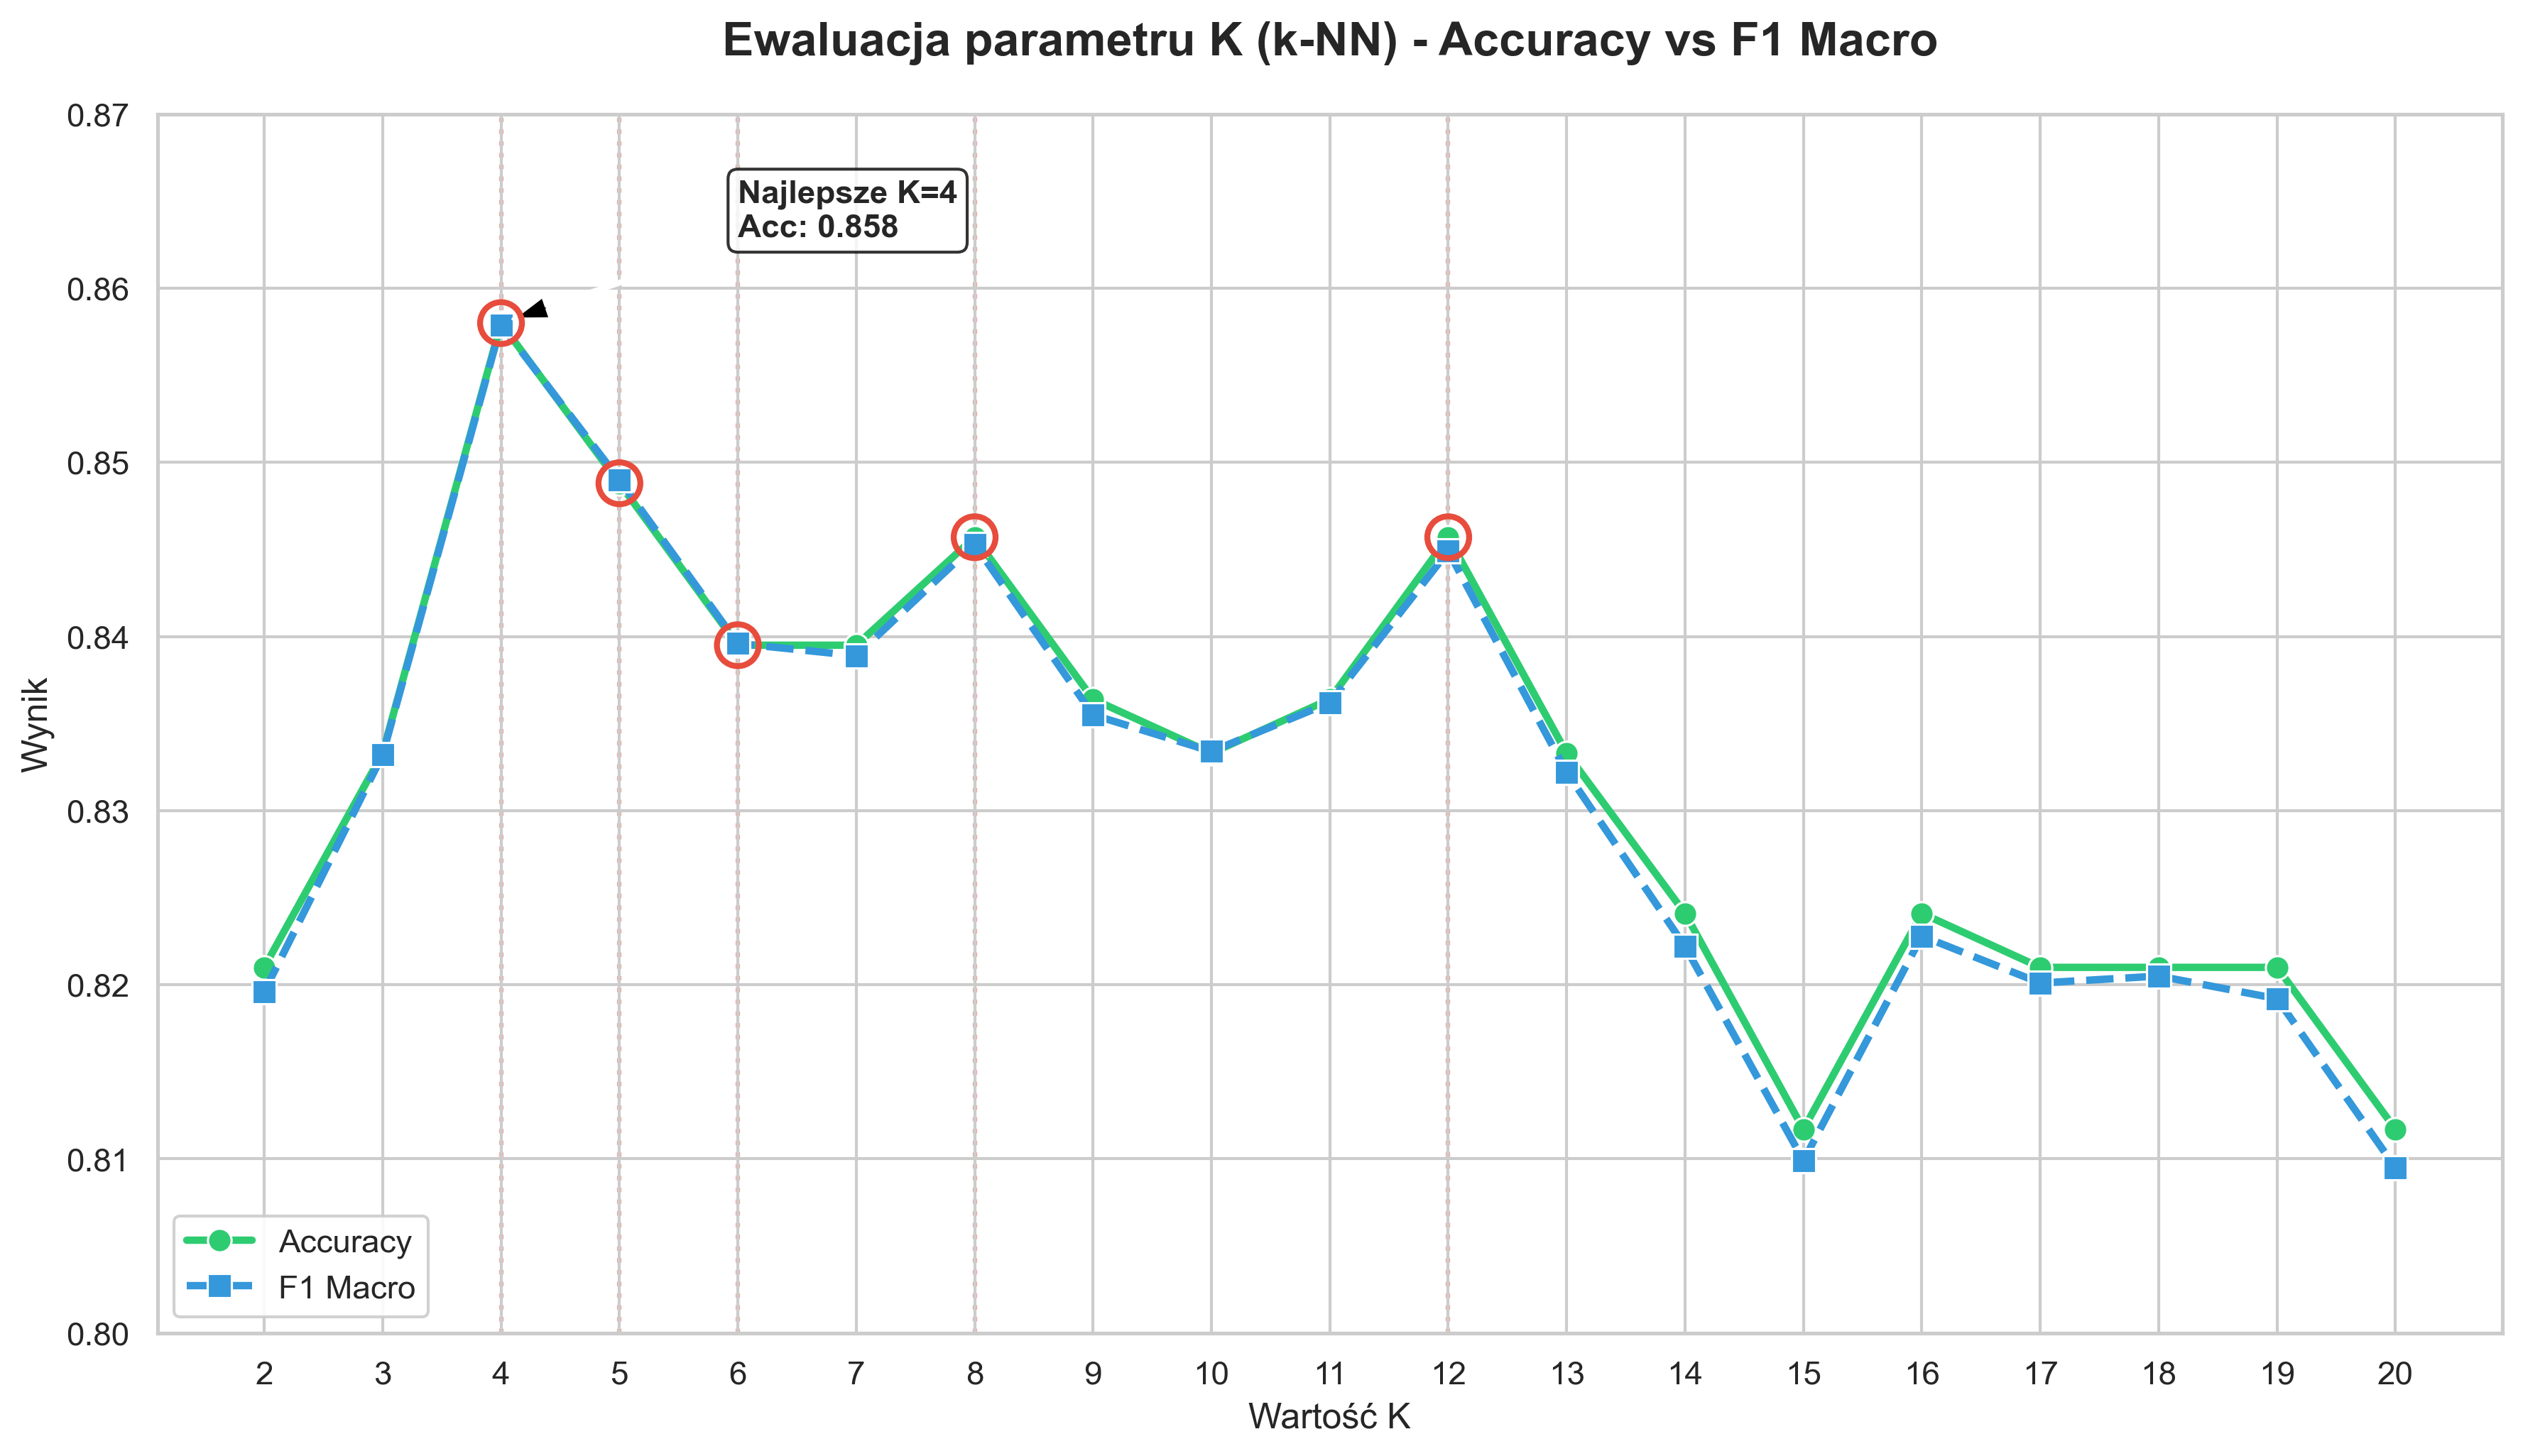
\includegraphics[width=0.9\textwidth]{public/wykres_knn.png} 
    \caption{Ewaluacja parametru k (k-NN) -- dokładność (\english{accuracy}) oraz F1-makro (\english{F1-macro}). Najlepsze wyniki uzyskano dla $k=4$.
    Czerwonymi okręgami zaznaczono pięć najlepszych wyników pod względem dokładności.}
    \label{fig:knn_eval}
\end{figure}

% TODO - wykres jako wykres + odwołania i opis
% TODO - tabelka jako tabelka

Eksperyment wykazał, że najwyższą dokładność uzyskano dla parametru $k \in \{4, 5, 6, 8, 12\}$. Należy jednak zaznaczyć, że rozpiętość wyników dokładności wyniosła ok. $0{,}05$, co przy ograniczonej liczebności zbioru testowego ($40$ przykładów na końcówkę) nakazuje zachować ostrożność w~interpretacji istotności tych różnic. 

Dodatkowo, dla tego samego zbioru danych, zweryfikowano podejście oparte na centroidach. Metoda ta niespodziewanie osiągnęła najwyższe wyniki zarówno pod względem dokładności, jak i~miary F1, co przedstawiono w Tabeli~\ref{tab:top_configurations}.

\begin{table}[H]
    \centering
    \caption{6 najlepszych konfiguracji wg. dokładności.}
    \label{tab:top_configurations}
    \begin{tabular}{|c|c|c|}
        \hline
        \textbf{k} & \textbf{dokładność} & \textbf{F1-makro} \\ 
        \hline
        centroid & $0{,}8735$ & $0{,}8736$ \\ 
        \hline
        4 & $0{,}8580$ & $0{,}8579$ \\ 
        \hline
        5 & $0{,}8488$ & $0{,}8490$ \\ 
        \hline
        8 & $0{,}8457$ & $0{,}8453$ \\ 
        \hline
        12 & $0{,}8457$ & $0{,}8449$ \\ 
        \hline
        6 & $0{,}8395$ & $0{,}8396$ \\ 
        \hline
    \end{tabular}
\end{table}

\subsection{Regularyzacja modelu poprzez zespołowe głosowanie}

W uczeniu maszynowym regularyzacja jest procesem wprowadzania dodatkowych ograniczeń w celu zapobiegania przeuczeniu (\english{overfitting}) i poprawy zdolności modelu do generalizacji \cite{goodfellow2016}. W kontekście modeli opartych na sąsiedztwie ryzyko to objawia się dwojako:

\begin{itemize}
    \item Dla małych wartości $k$ (np. $k=1$), model wykazuje wysoką wariancję i jest nadmiernie wrażliwy na szum.
    \item Dla dużych wartości $k$, następuje wzrost obciążenia (\textit{bias}) i zjawisko niedouczenia (\textit{underfitting}).
\end{itemize}


W celu optymalizacji kompromisu między obciążeniem a wariancją (\textit{bias-variance tradeoff}), w~architekturze systemu \definicja{Moje Konie} zrezygnowano z deterministycznego wyboru pojedynczej wartości parametru $k$ na rzecz podejścia zespołowego (\english{ensemble learning}). Skonstruowany model finalny funkcjonuje jako komitet klasyfikatorów $\mathcal{M}$, w skład którego wchodzą algorytmy $k$-NN dla $k \in \{4, 5, 6, 8, 12\}$ oraz klasyfikator oparty na centroidach kategorii.

Ostateczna decyzja klasyfikacyjna podejmowana jest w procedurze głosowania większościowego (\textit{majority voting}). Formalnie, wybór końcowej intencji $I_{final}$ definiuje się jako zadanie poszukiwania argumentu maksymalizującego liczbę wskazań w całym zespole:

\begin{equation}
    I_{final} = \argmax_{i \in \text{Intencje}} \sum_{m \in \mathcal{M}} \mathbbm{1}(P_m(q) = i)
\end{equation}

gdzie:
\begin{itemize}
    \item $\mathcal{M}$ -- zbiór modeli składowych (klasyfikatory $k$-NN oraz model centroidów),
    \item $P_m(q)$ -- intencja wskazana przez $m$-ty klasyfikator dla zapytania $q$,
    \item $\mathbbm{1}(\cdot)$ -- funkcja wskaźnikowa przyjmująca wartość 1, gdy warunek jest spełniony.
\end{itemize}

W sytuacjach spornych, gdy co najmniej dwie intencje uzyskają identyczną liczbę głosów, algorytm aplikuje heurystykę rozstrzygającą (\textit{tie-breaker}). Polega ona na porównaniu skumulowanej wiarygodności (\textit{confidence score}), obliczanej jako suma podobieństw cosinusowych zwróconych przez te modele z komitetu, które wskazały daną klasę:

\begin{equation}
    S_i = \sum_{m \in \mathcal{M}_i} \text{sim}(q, \text{ref}_m)
\end{equation}

gdzie $\mathcal{M}_i$ to podzbiór modeli głosujących na intencję $i$, a $\text{sim}(q, \text{ref}_m)$ oznacza podobieństwo cosinusowe zapytania do najbliższych sąsiadów lub centroidu w danym modelu. Zwycięża klasa o~najwyższej wartości $S_i$, co premiuje intencję o większej lokalnej gęstości semantycznej lub silniejszym powiązaniu ze środkiem ciężkości kategorii.


Zastosowana strategia znajduje uzasadnienie w teorii uczenia zespołowego. Jak wskazuje Dietterich \cite{dietterich2000}, uśrednianie wyników wielu modeli pozwala zredukować ryzyko wyboru błędnej hipotezy. W projektowanym systemie głosowanie między modelami o zróżnicowanej „ziarnistości” pełni rolę niejawnej regularyzacji, stabilizując predykcję w obszarach niejednoznacznych semantycznie.

Ewaluacja końcowa modelu zespołowego (\english{ensemble}) wykazała wyniki przedstawione w~Tabeli~\ref{tab:final_results}. Choć są one marginalnie niższe w porównaniu do najlepszych konfiguracji pojedynczych (Tabela~\ref{tab:top_configurations}), spadek ten uznano za pomijalny koszt regularyzacji. Zwiększona stabilność predykcji daje bowiem silniejsze podstawy do prognozowania wysokiej skuteczności systemu w~środowisku produkcyjnym.

\begin{table}[H]
    \centering
    \caption{Wyniki końcowe modelu zespołowego (\english{ensemble}) po regularyzacji}
    \label{tab:final_results}
    \begin{tabular}{|l|c|}
        \hline
        \textbf{Metryka} & \textbf{Wynik} \\ 
        \hline
	    Dokładność & $0{,}854$ \\ 
        \hline
	    F1-makro & $0{,}855$ \\ 
        \hline
    \end{tabular}
\end{table}
% TODO - dokładniej opisać
% uwaga: Centroid - jakoś trzeba byłoby to opisać
% uwaga: ważonego - procesie głosowania ważonego - czym? jak dokładnie wygląda ta procedura


\subsection{Analiza błędów i kierunki rozwoju architektury}

Ostateczną weryfikację skuteczności wdrożonego rozwiązania stanowi analiza macierzy pomyłek (\english{confusion matrix}), przedstawionej na Rysunku~\ref{fig:macierz_pomylek}. Pozwala ona nie tylko na ocenę globalnej precyzji, ale przede wszystkim na zidentyfikowanie semantycznych ,,obszarów ryzyka'', w których model ma trudności z poprawną separacją klas.

\begin{figure}%[H]
    \centering
    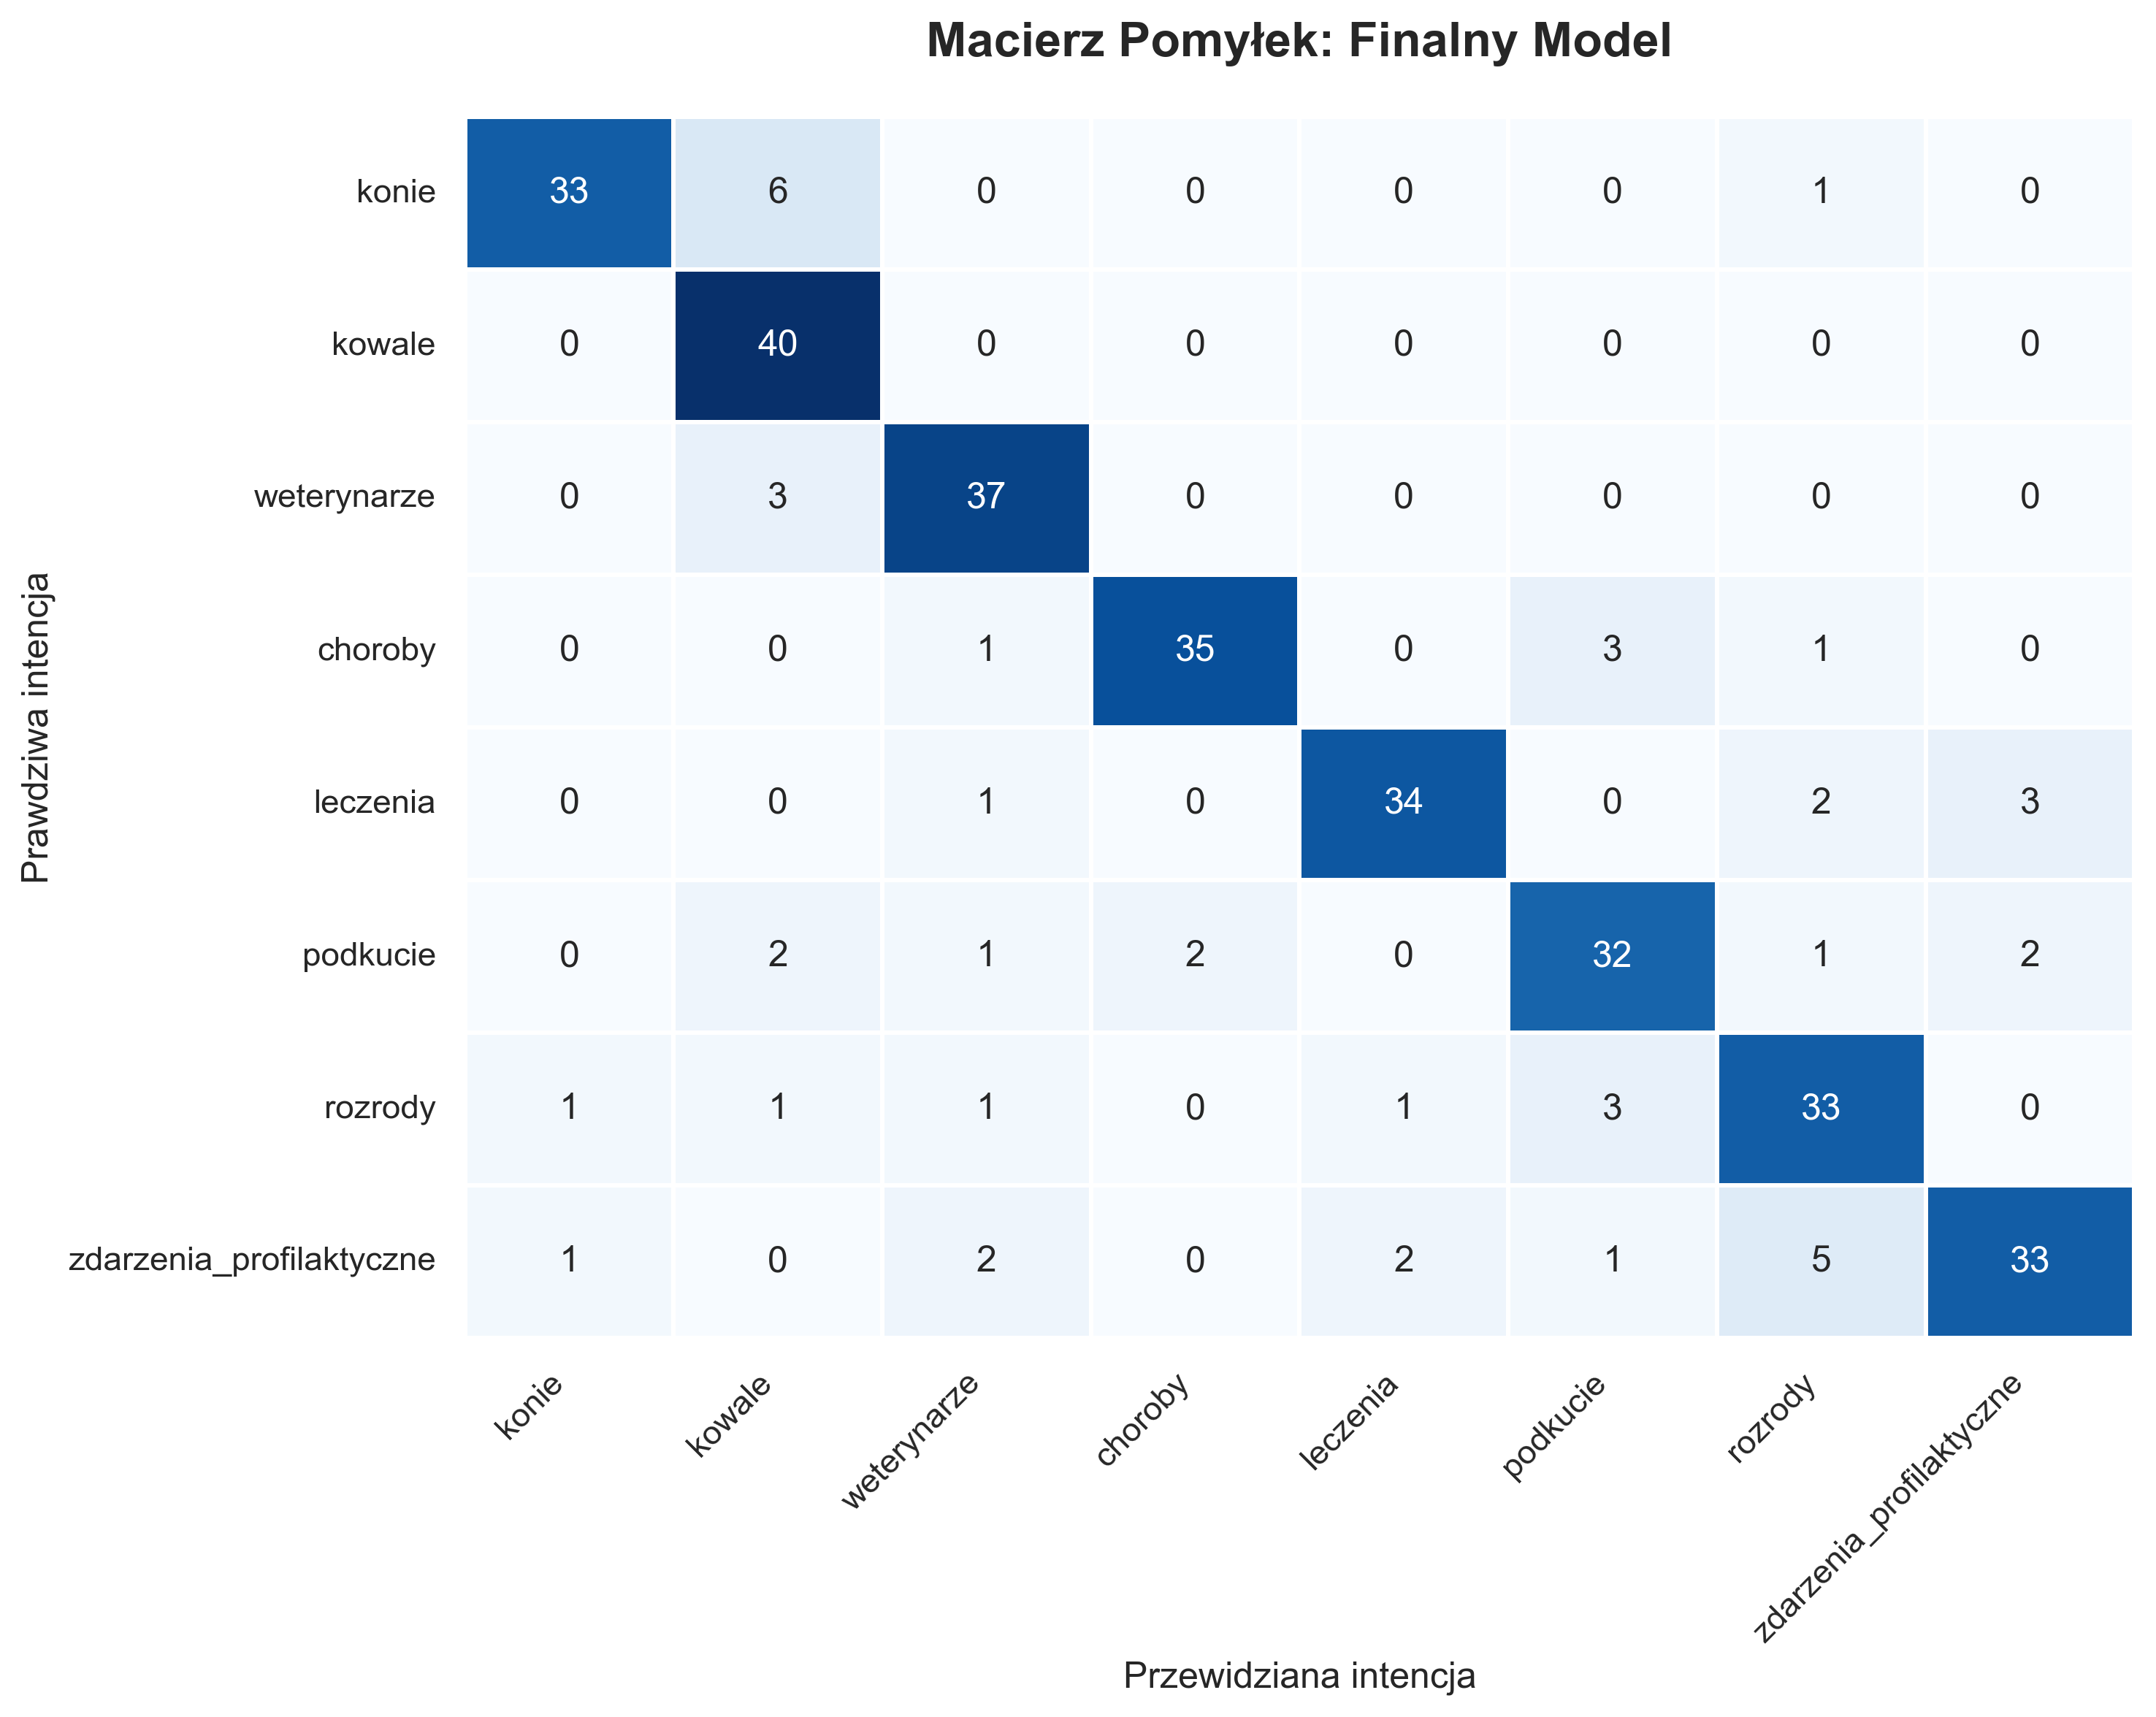
\includegraphics[width=0.9\textwidth]{public/macierz_pomylek.png} 
    \caption{Macierz pomyłek dla finalnego modelu w środowisku produkcyjnym.}
    \label{fig:macierz_pomylek}
\end{figure}

Szczegółowa inspekcja wyników prowadzi do następujących wniosków:

\begin{description}
	\item[Wysoka precyzja dla encji rzadkich:] Intencja \texttt{kowale} została rozpoznana bezbłędnie (40/40 przypadków). Sugeruje to, że słownictwo związane z tą profesją jest silnie dystynktywne w~przestrzeni wektorowej. Jednakże, zauważalna jest pewna asymetria – intencja \texttt{konie} była mylona z intencją \texttt{kowale} aż w 6 przypadkach. Może to wynikać z konstrukcji zdaniowych, gdzie imię konia występuje w bliskim sąsiedztwie słowa kluczowego oznaczającego specjalistę.
    
	\item[Nakładanie się kontekstów medycznych:] Największe rozproszenie błędów widoczne jest w~grupie intencji weterynaryjnych: \texttt{choroby}, \texttt{leczenia} oraz \texttt{zdarzenia\_profilaktyczne}. Jest to zjawisko oczekiwane, wynikające z naturalnego podobieństwa semantycznego (np. szczepienie jest zarówno procedurą medyczną, jak i elementem profilaktyki).
    
	\item[Interferencja profilaktyki i rozrodu:] Istotnym błędem jest mylenie intencji \texttt{zdarzenia\_\allowbreak{}profi\allowbreak{}laktyczne} z \texttt{rozrodami} (5 pomyłek). Wskazuje to na konieczność doprecyzowania bazy wiedzy o frazy rozróżniające opiekę nad źrebięciem (profilaktyka) od procesów hodowlanych w kolejnych etapach rozwoju proejktu.
\end{description}

\paragraph{Rekomendacje dla rozwoju systemu:}~\\
Analiza powyższych błędów wyznacza jasny kierunek dalszej optymalizacji. Przyszłe prace nad klasyfikatorem intencji powinny skupić się na:
\begin{enumerate}
    \item \textbf{Wzbogaceniu bazy wzorców o trudne przypadki:} Dodaniu do bazy wiedzy tych specyficznych sformułowań, które model obecnie myli. Pozwoli to systemowi lepiej nauczyć się subtelnych różnic między podobnymi klasami (np. skuteczniej odróżniać opisy koni od zapytań o kowala).
    \item \textbf{Klasyfikacji hierarchicznej:} Rozważeniu architektury dwuetapowej, gdzie model najpierw rozróżnia szerokie domeny (np. \textit{Operacje Cykliczne} vs \textit{Zdrowie}), a dopiero w drugim kroku precyzuje konkretną końcówkę. Pozwoliłoby to na zredukowanie szumu informacyjnego wewnątrz gęstego klastra intencji medycznych.
\end{enumerate}

Podsumowując, mimo wskazanych obszarów do poprawy, model osiąga stabilność operacyjną wystarczającą do wdrożenia w ramach sytemu \definicja{Moje Konie} i jego części \definicja{Asystenta NLP} 

\chapter{Opracowanie i ocena eksperymentalna metody wypełniania żądań REST}

\section{Inżynieria zapytań}

Proces opracowania metody automatycznego mapowania wypowiedzi użytkownika w języku naturalnym na strukturalne żądania w formacie JSON, zgodne z interfejsem programistycznym aplikacji typu REST, miał charakter iteracyjny. Takie podejście jest zgodne z iteracyjnym paradygmatem rozwoju systemów generatywnej sztucznej inteligencji (\english{Generative AI}), opisywanym w literaturze jako kluczowy element poprawy jakości wnioskowania wnioskowania dużych modeli językowych (\akronim{LLM}) \cite{brown2020language,ouyang2022training}. Ewolucja zastosowanych metod obejmowała przejście od prostych strategii, umożliwiających wnioskowanie bez dostarczonych przykładów (\english{Zero-Shot}), do bardziej zaawansowanych technik, które dzięki wykorzystaniu niewielkiej liczby reprezentatywnych przykładów (\english{Few-Shot Prompting}), pozwalają precyzyjniej ukierunkować model i znacząco zwiększyć poprawność generowanych struktur \cite{brown2020language,liu2023pre}.

W początkowej fazie eksperymentów skoncentrowano się na testowaniu możliwości \definicja{dużych modeli językowych} (\akronim{LLM}, \english{Large Language Models}) bez wykorzystania dodatkowego klasyfikatora intencji. Przyjęto wówczas założenie, że model o wystarczająco dużej liczbie parametrów będzie w~stanie samodzielnie zidentyfikować cel użytkownika, dobrać odpowiedni punkt końcowy (\english{endpoint}) oraz dokonać ekstrakcji danych. W tym celu opracowano zapytanie (\english{prompt}), które zawierało opis struktury bazy danych oraz ścisłe żądanie zwrotu odpowiedzi w formacie JSON.

\subsection{Konstrukcja pierwszego zapytania}

Pierwotna konstrukcja zapytania charakteryzowała się znaczną długością, co wynikało z konieczności zawarcia w jednym zapytaniu pełnej wiedzy o architekturze systemu. W praktyce oznaczało to bezpośrednie włączenie do promptu zarówno aktualnego stanu bazy danych dla danej hodowli, jak i wybranych fragmentów dokumentacji OpenAPI, które odzwierciedlały definicje obiektów oraz dostępnych punktów końcowych. Na wykazie \ref{wyk:prompt_verbatim} przedstawiono strukturę tego zapytania, które składało się z kilku kluczowych sekcji:

\newpage
\begin{wykaz}[ht]
    \centering
    \begin{tcolorbox}[colback=gray!5, colframe=gray!50, arc=0mm, boxrule=0.5pt]
        \begin{verbatim}
Schemat danych wejściowych (format JSON): {schema_prompt}

Twoim zadaniem jest wygenerować obiekt w formacie JSON zgodny z powyższym schematem danych wejściowych na podstawie opisu użytkownika. 

Aktualny stan bazy danych: {stan}
Użytkownik: {prompt}

Odpowiedź w formacie JSON:
        \end{verbatim}
    \end{tcolorbox}
    \caption{Struktura pierwotnego zapytania zawierająca pełny schemat bazy danych.}
    \label{wyk:prompt_verbatim}
\end{wykaz}

\begin{itemize}
    \item \textbf{Definicja schematu danych wejściowych:} sekcja \texttt{\{schema\_prompt\}} zawiera pełny opis struktur JSON dla wszystkich obsługiwanych punktów końcowych systemu. Dzięki temu model ma pełną wiedzę o formacie danych, jednak konieczne jest przetwarzanie wielu tabel i pól, często niezwiązanych z aktualnym zapytaniem.
    \item \textbf{Instrukcja zadania:} polecenie sugeruje wygenerowanie obiektu JSON na podstawie opisu użytkownika, zgodnie ze schematem i aktualnym stanem bazy.
    \item \textbf{Aktualny stan bazy danych:} sekcja \texttt{\{stan\}} zawiera bieżące informacje o obiektach w systemie (np. konie, kowale, weterynarze). Model może wykorzystywać te dane do wypełnienia odpowiednich pól i odwołań w JSON.
    \item \textbf{Użytkownik:} sekcja \texttt{\{prompt\}} przekazuje opis, zapytanie lub wymagania użytkownika, które mają zostać odwzorowane w formacie JSON.
\end{itemize}

Zbiorcze wyniki tej fazy testów przedstawia tabela \ref{tab:llm_comparison1}. Analiza danych wskazuje na niską skuteczność podejścia \textit{Zero-Shot}. Uzyskane wyniki pozwalają domniemywać, że przyczyną tego stanu rzeczy jest rozproszenie mechanizmu uwagi (\english{attention}) modelu na zbyt rozbudowanym opisie schematu.

Testom eksperymentalnym poddano wybrane duże modele językowe, obejmujące zarówno modele komercyjne, jak i otwartoźródłowe. Wśród nich znalazły się: 
\begin{description}
    \item[GPT-4o] (\definicja{OpenAI}) -- zaawansowany model komercyjny, optymalizowany pod kątem wielomodalności i wysokiej precyzji w zadaniach logicznych. \textbf{Typ:} Zamknięty (SaaS).
    
    \item[DeepSeek-V3] (\definicja{DeepSeek}) -- model o otwartej architekturze, charakteryzujący się wysoką wydajnością obliczeniową i zoptymalizowanym kosztem inferencji. \textbf{Typ:} Otwartoźródłowy (\english{Open-weights}).
    
    \item[Gemini 1.5 Flash] (\definicja{Google}) -- model komercyjny zoptymalizowany pod kątem zaawansowanego rozumowania językowego oraz przetwarzania złożonych danych wejściowych w formacie wielomodalnym. \textbf{Typ:} Zamknięty (SaaS).
\end{description}

W celu obiektywnej oceny jakości generowanych odpowiedzi zdefiniowano trzy kluczowe miary eksperymentalne:
\begin{itemize}
    \item \textbf{Skuteczność (\english{Effectiveness}):} mierzona binarnie (0 lub 1). Wartość 1 oznacza poprawną identyfikację docelowego punktu końcowego (\english{endpoint selection}), natomiast 0 wskazuje na wybór błędnego adresu URL.
    \item \textbf{Precyzja (\english{Precision}):} mierzona w znormalizowanym zakresie od 0 do 1. W badaniu przyjęto model oceny oparty na płaskiej strukturze par klucz-wartość, co wynika z braku zagnieżdżeń w testowanych schematach. Miara ta obliczana jest jako stosunek liczby poprawnie odwzorowanych elementów do sumy wszystkich unikatowych kluczy obecnych zarówno w~obiekcie wzorcowym, jak i wygenerowanym. W praktyce oznacza to, że wynik jest obniżany w~trzech przypadkach: gdy model pominie wymagany klucz, gdy przypisze mu błędną wartość lub gdy wygeneruje dodatkowe, nadmiarowe klucze spoza schematu. Wartość 1 oznacza idealną zgodność struktury i treści, natomiast 0 oznacza całkowity brak wspólnych elementów.
    \item \textbf{Efektywność (\english{Efficiency}):} wskaźnik binarny weryfikujący poprawność operacyjną wygenerowanego żądania. Wartość 1 (sukces) przypisywana jest w przypadku otrzymania kodu odpowiedzi z grupy 2xx protokołu HTTP, co potwierdza pomyślne przejście walidacji schematu oraz trwały zapis danych w bazie. Wartość 0 oznacza błąd po stronie klienta (np.~błąd struktury 4xx) lub błąd serwera (5xx), uniemożliwiający realizację żądania.
\end{itemize}

%Precyzja i efektywność liczona tylko dla poprawnie zdefiniowanych endpointów, w przeciwnym przypadku nie była liczona czy jak robimy?

Wszystkie testy eksperymentalne przeprowadzono w oparciu o zestaw przygotowanych endpointów REST, odpowiadających głównym obszarom funkcjonalnym systemu. Wśród obsługiwanych endpointów znalazły się: \texttt{/api/konie} (zarządzanie stadem), \texttt{/api/wydarzenia/rozrody} (rozród), \texttt{/api/wydarzenia/zdarzenia\_profilaktyczne} (profilaktyka), \texttt{/api/wydarzenia/podkucie} (pielęgnacja kopyt), \texttt{/api/wydarzenia/leczenia} i \texttt{/api/wydarzenia/choroby} (weterynaria i zdrowie) oraz \texttt{/api/kowale} i \texttt{/api/weterynarze} (zarządzanie kontaktami do specjalistów).

Dla każdego z tych endpointów opracowano 20 przykładowych scenariuszy użycia, które stanowiły zestaw danych testowych. Scenariusze te zostały przygotowane ręcznie przez członków zespołu badawczego i obejmowały typowe zapytania użytkowników, w tym zarówno poprawne, jak i potencjalnie problematyczne przypadki danych. Dzięki temu wyniki eksperymentów odzwierciedlają zdolność modeli do generowania poprawnych struktur JSON w podejściu Zero-Shot, bez wcześniejszego uczenia na konkretnych przykładach.

Aby zwiększyć stabilność wyników i ograniczyć wpływ losowości generatywnych modeli, każde zapytanie testowe zostało wykonane pięciokrotnie dla wszystkich badanych modeli. Ostateczne wyniki przedstawiono jako średnią z tych pięciu powtórzeń, co pozwala czytelnikowi na ocenę powtarzalności odpowiedzi modeli oraz zapewnia wiarygodność prezentowanych miar skuteczności, precyzji i efektywności. Takie podejście pozwoliło zarówno na obiektywną ocenę jakości generowanych struktur JSON, jak i na identyfikację potencjalnych problemów związanych z halucynacjami modeli czy niejednoznacznością interpretacji zapytań użytkowników.

\begin{table}[h!]
\centering
\caption{Wyniki wstępnej oceny eksperymentalnej modeli LLM (podejście Zero-Shot)}
\label{tab:llm_comparison1}
\begin{tabular}{|l|c|c|c|c|}
\hline
\textbf{Model} & \textbf{Skuteczność} & \textbf{Śr. Precyzja} & \textbf{Efektywność} \\ \hline
GPT-4o         & 0,34                 & 0,28                  & 0,41                 \\ \hline
DeepSeek-V3    & 0,45                 & 0,34                  & 0,45                 \\ \hline
Gemini 1.5 Flash & 0,41               & 0,39                  & 0,44                 \\ \hline
\end{tabular}
\end{table}

Wstępne wyniki pokazały, że podejście \textit{Zero-Shot} generuje liczne halucynacje, szczególnie w~zakresie identyfikatorów relacyjnych. Modele często tworzyły nieistniejące numery ID lub błędnie interpretowały polskie nazewnictwo fachowe stosowane w hodowli koni, co bezpośrednio obniżało miarę precyzji i efektywności. Przykładowo, model potrafił poprawnie wybrać endpoint (skuteczność=1), lecz z wstawiał losowe klucze obce, co skutkowało odrzuceniem żądania przez backend (efektywność wynosząca 0).

\subsection{Wykorzystanie technik inżynierii zapytań}

Wraz z rozwojem badań nad modelami generatywnymi istotnym elementem stało się opracowanie skutecznych technik inżynierii zapytań (\english{prompt engineering}). W literaturze \cite{liu2023pre,zhou2023comprehensive} podkreśla się, że poprawne konstruowanie zapytań może znacząco wpływać na jakość odpowiedzi LLM, szczególnie w zadaniach wymagających precyzyjnej struktury odpowiedzi lub wnioskowania na podstawie złożonych danych. Do kluczowych technik należą m.in.: stosowanie jednoznacznych instrukcji i jasnych ograniczeń formalnych, minimalizowanie niejednoznaczności poprzez kontekstowe doprecyzowanie roli modelu, przekazywanie przykładów poprawnych odpowiedzi (metody \english{Few-Shot}), stosowanie formatów szablonowych oraz technik sugerujących strukturę wyjścia (np. „Odpowiadaj WYŁĄCZNIE w poprawnym formacie JSON”). Praktyki te pozwalają ograniczyć halucynacje modeli, zwiększyć stabilność generowanych odpowiedzi oraz poprawić zgodność wyników z oczekiwaniami systemu wykonawczego.

\newpage
\begin{wykaz}[ht]
    \centering
    \begin{tcolorbox}[colback=gray!5, colframe=gray!50, arc=0mm, boxrule=0.5pt]
        \begin{verbatim}
ROLA:
Jesteś systemem przetwarzania zapytań użytkownika na poprawne struktury JSON
zgodne z interfejsem REST. Twoim zadaniem jest dokładna analiza opisu oraz
wygenerowanie wyłącznie poprawnego obiektu JSON zgodnego ze schematem danych.

ZASADY:
1. Odpowiadaj WYŁĄCZNIE w poprawnym formacie JSON.
2. Nie dodawaj żadnych pól, kluczy ani wartości, które nie występują w schemacie.
3. Jeśli użytkownik opisuje dane niezgodne ze schematem - pomiń je.
4. Jeśli użytkownik podaje wartość niepoprawną typologicznie - dopasuj ją do schematu,
ale nie zgaduj wartości niepodanych.
5. Nie generuj tekstu objaśniającego ani komentarzy.
6. Wybierz najbardziej pasujący endpoint REST na podstawie struktury danych.
7. Analizuj problem krok po kroku (nie wyświetlaj rozumowania) i dopiero potem wygeneruj JSON.
8. Jeśli dane mają odwołanie do istniejących obiektów, używaj wartości ze stanu bazy.
9. W przypadku niejednoznaczności wybierz najprostsze poprawne rozwiązanie.


SCHEMAT DANYCH (JSON):
{schema_prompt}

AKTUALNY STAN BAZY:
{stan}

UŻYTKOWNIK:
{prompt}

WYNIK:
Zwróć obiekt JSON zawierający:
{
"endpoint": "<wybrany_endpoint>",
"data": <wygenerowany_json>
}
        \end{verbatim}
    \end{tcolorbox}
    \caption{Struktura pierwotnego zapytania zawierająca pełny schemat bazy danych.}
    \label{wyk:zero-shot-prompt-engineering}
\end{wykaz}

\begin{table}[h!]
\centering
\caption{Wyniki eksperymentalne z wykorzystaniem technik inżynierii zapytań}
\label{tab:llm_comparison2}
\begin{tabular}{|l|c|c|c|}
\hline
\textbf{Model} & \textbf{Skuteczność} & \textbf{Śr. Precyzja} & \textbf{Efektywność} \\ \hline
GPT-4o & 0,62 & 0,57 & 0,65 \\ \hline
DeepSeek-V3 & 0,55 & 0,51 & 0,57 \\ \hline
Gemini 1.5 Flash & 0,59 & 0,54 & 0,60 \\ \hline
\end{tabular}
\end{table}


Analiza wyników przedstawionych w tabeli \ref{tab:llm_comparison2} wskazuje, że udoskonalone zapytanie Zero-Shot znacząco poprawiło skuteczność i precyzję generowanych odpowiedzi w porównaniu z pierwotnym podejściem (Tabela \ref{tab:llm_comparison1}). Modele rzadziej generowały nieistniejące identyfikatory i lepiej odwzorowywały strukturę danych zgodnie z wybranym schematem endpointu, co przełożyło się na poprawne wykonanie żądania w systemie REST.

\subsection{Strategia Few-Shot Prompting}

Doświadczenia z~podejściem bazowym stały się bezpośrednim impulsem do wdrożenia strategii \textit{Few-Shot Prompting}. Nowa architektura zapytania (Wykaz \ref{wyk:few-shot}) została wzbogacona o~sekwencję par przykładów uczących, co pozwoliło modelowi na interpretację intencji użytkownika na podstawie konkretnych wzorców, a~nie tylko abstrakcyjnego opisu technicznego. Dzięki temu \definicja{duży model językowy} zyskał punkt odniesienia w~zakresie oczekiwanej struktury obiektu \textsf{JSON} oraz sposobu mapowania potocznych sformułowań na parametry funkcji \akronim{API}.

\begin{wykaz}[ht]
    \centering
    \begin{tcolorbox}[colback=gray!5, colframe=gray!50, arc=0mm, boxrule=0.5pt]
        \begin{verbatim}
ROLA:
Jesteś systemem przetwarzania zapytań użytkownika na poprawne struktury JSON
zgodne z interfejsem REST. Twoim zadaniem jest dokładna analiza opisu oraz
wygenerowanie wyłącznie poprawnego obiektu JSON zgodnego ze schematem danych.


ZASADY:
1. Odpowiadaj WYŁĄCZNIE w poprawnym formacie JSON.
2. Nie dodawaj żadnych pól, kluczy ani wartości, które nie występują w schemacie.
3. Jeśli użytkownik opisuje dane niezgodne ze schematem – pomiń je.
4. Jeśli użytkownik podaje wartość niepoprawną typologicznie – dopasuj ją do schematu,
ale nie zgaduj wartości niepodanych.
5. Nie generuj tekstu objaśniającego ani komentarzy.
6. Wybierz najbardziej pasujący endpoint REST na podstawie struktury danych.
7. Analizuj problem krok po kroku (nie wyświetlaj rozumowania) i dopiero potem wygeneruj JSON.
8. Jeśli dane mają odwołanie do istniejących obiektów, używaj wartości ze stanu bazy.
9. W przypadku niejednoznaczności wybierz najprostsze poprawne rozwiązanie.


SCHEMAT DANYCH (JSON):
{schema_prompt}


AKTUALNY STAN BAZY:
{stan}


% Pętla generująca przykłady few-shot:
for train in examples_train:
  Użytkownik: {train_prompt}
  WYNIK:
  Zwróć obiekt JSON zawierający:
  {
  "endpoint": "<wybrany_endpoint>",
  "data": <wygenerowany_json>
  }
% Koniec pętli

UŻYTKOWNIK:
{prompt}


WYNIK:
Zwróć obiekt JSON zawierający:
{
"endpoint": "<wybrany_endpoint>",
"data": <wygenerowany_json>
}
        \end{verbatim}
    \end{tcolorbox}
    \caption{Struktura zapytania zawierająca pełny schemat bazy danych i przykłady uczące.}
    \label{wyk:few-shot}
\end{wykaz}

Wykaz \ref{wyk:few-shot} przedstawia szablon zapytania. Fragmenty ujęte w nawiasy klamrowe (np. \texttt{{stan}}) oraz instrukcje sterujące (pętla \texttt{for}) stanowią elementy dynamiczne, które są automatycznie uzupełniane danymi z systemu przed wysłaniem zapytania do modelu. Struktura zoptymalizowanego zapytania w~podejściu \textit{Few-Shot} zachowała kluczowe sekcje z~poprzedniej iteracji, wzbogacając je~o~moduł demonstracyjny dla modelu. Elementy takie jak definicja schematu danych oraz ogólna instrukcja zadania pozostały identyczne jak w~przypadku metody \textit{Zero-Shot}, co pozwoliło na rzetelne porównanie wpływu samych przykładów na jakość generowanych odpowiedzi:

\begin{description}
    \item \textbf{Definicja schematu danych:} sekcja \texttt{\{schema\_prompt\}} zawiera kompletny opis struktury \textsf{JSON} dla wybranego endpointu, określający wymagane i opcjonalne pola oraz typy danych. Dzięki temu model ma pełną wiedzę o formacie odpowiedzi, jednocześnie ograniczając konieczność przetwarzania informacji niezwiązanych z bieżącym zapytaniem użytkownika.
    \item \textbf{Instrukcja zadania:} jasne polecenie sugeruje modelowi wygenerowanie obiektu \textsf{JSON} w oparciu o opis użytkownika oraz dane ze stanu bazy, bez dodawania pól ani wartości spoza schematu. Model ma również korzystać z dostępnych danych referencyjnych w bazie przy wypełnianiu powiązań.
    \item \textbf{Przykłady uczące (Few-Shot):} sekcja iteracyjnie wstawiająca pary \texttt{\{train\_prompt\}} i \texttt{\{train\_json\}}. Te przykłady służą jako wzorzec poprawnego mapowania opisów użytkownika na struktury \textsf{JSON}, pomagając modelowi uniknąć błędów logicznych i halucynacji przy generowaniu nowych zapytań.
    \item \textbf{Aktualny stan bazy danych:} sekcja \texttt{\{stan\}} przekazuje bieżące informacje o obiektach systemu (np. konie, kowale, weterynarze), które mogą być wykorzystywane do wypełniania powiązań i wartości w generowanym \textsf{JSON}.
    \item \textbf{Użytkownik:} sekcja \texttt{\{prompt\}} zawiera aktualne zapytanie lub opis użytkownika, które mają zostać odwzorowane w formacie \textsf{JSON}.
\end{description}

\begin{table}[h!]
\centering
\caption{Wyniki wstępnej oceny eksperymentalnej modeli LLM (podejście Few-Shot)}
\label{tab:llm_few_shot}
\begin{tabular}{|l|c|c|c|c|}
\hline
\textbf{Model} & \textbf{Skuteczność} & \textbf{Śr. Precyzja} & \textbf{Efektywność} \\ \hline
GPT-4o         & 0,74                 & 0,68                  & 0,79                 \\ \hline
DeepSeek-V3    & 0,81                 & 0,64                  & 0,65                 \\ \hline
Gemini 1.5 Flash & 0,81               & 0,84                  & 0,79                 \\ \hline
\end{tabular}
\end{table}

Zbiorcze wyniki oceny modeli w~podejściu \textit{Few-Shot} (Tabela \ref{tab:llm_few_shot}) potwierdziły znaczącą przewagę tej metody nad próbami \textit{Zero-Shot}. Na szczególną uwagę zasługują wyniki modelu \textbf{Gemini 1.5 Flash}, który wykazał się najwyższą średnią precyzją ($0,84$), zachowując przy tym wysoką skuteczność ($0,81$) oraz satysfakcjonującą efektywność ($0,79$). Połączenie tych cech czyni go optymalnym silnikiem dla projektowanego \definicja{Asystenta NLP} w~kontekście stabilności struktury wyjściowej JSON.

% TODO: dodać front pareto

Warto zaznaczyć, że modele \textit{Gemini 1.5 Flash} oraz \textit{DeepSeek-V3} posiadały istotną przewagę implementacyjną w stosunku do modelu \textit{GPT-4o}. Ze względu na brak dostępu do interfejsu programistycznego dla tego ostatniego, testy mogły być przeprowadzane wyłącznie w trybie interaktywnym za pośrednictwem przeglądarki. Pozostałe modele umożliwiały natomiast pełną automatyzację oraz integrację z potokiem przetwarzania danych, a także precyzyjną kontrolę parametrów generowania odpowiedzi, takich jak stopień losowości czy szczegółowość wygenerowanego tekstu. W kontekście systemów produkcyjnych działających w czasie rzeczywistym możliwość programistycznego wywołania modelu okazała się kluczowym czynnikiem przy wyborze końcowej technologii.

W toku prac wdrożeniowych nastąpiła konieczność migracji z modelu \textit{Gemini 1.5 Flash} na nowszą wersję \textit{Gemini 2.5 Flash}. Zmiana ta była podyktowana decyzją dostawcy o wyłączeniu dostępu do interfejsu programistycznego starszej wersji modelu. Migracja, choć wymuszona czynnikami zewnętrznymi, pozwoliła na utrzymanie dotychczasowych wskaźników precyzji przy jednoczesnym zapewnieniu stabilności infrastrukturalnej systemu w długofalowej perspektywie eksploatacyjnej. Dzięki tak zaprojektowanej architekturze, opartej na modelu Gemini, system osiągnął wysoką deterministyczność przy zachowaniu naturalności interfejsu użytkownika.

W praktyce podejście to generowało kilka istotnych ograniczeń inżynierskich. Ze względu na wstrzykiwanie pełnej specyfikacji bazy danych do zapytania, jego długość była znaczna, a wraz ze wzrostem liczby obsługiwanych endpointów oraz rozrostem systemu, metoda stawała się coraz mniej skalowalna.

Dodatkowo, model musiał przetwarzać rozbudowany zbiór danych wejściowych, z którego znaczna część stanowiła informacyjny „szum”. Na przykład, przy prostym poleceniu typu „dodaj nowego konia”, model analizował jednocześnie schematy związane z leczeniem, kowalami, rozrodem czy profilaktyką, co prowadziło do nadmiernego obciążenia i zwiększało ryzyko pomyłki przy wyborze właściwego endpointu lub błędnej interpretacji danych.

Dodatkowym obciążeniem było wstrzykiwanie aktualnego stanu bazy danych dla wszystkich encji jednocześnie. Dane te nie tylko konsumowały dostępne okno kontekstowe (\english{context window}), ale również prowadziły do rzadszych, lecz trudnych do zdiagnozowania błędów semantycznych, w których model próbował powiązać dane użytkownika z nieprawidłowym kontekstem pochodzącym z innej części bazy. Doświadczenia te stały się bezpośrednim impulsem do wprowadzenia dedykowanego klasyfikatora, który pozwolił na selektywne ładowanie wyłącznie tych fragmentów schematu i danych, które są krytyczne dla realizacji konkretnego żądania.

%TODO: dodać referencję do rozdziału o klasyfikatorze intencji







\section{Dynamiczna inżynieria zapytań}

Fundamentem optymalizacji procesu generowania żądań było przejście od statycznych, jednolitych instrukcji do \definicja{dynamicznej inżynierii zapytań}. W nowym podejściu przykłady referencyjne są pobierane w czasie rzeczywistym z dedykowanego zbioru wzorców (\english{Few-Shot}), co zapewnia pełną zgodność generowanych odpowiedzi z aktualną specyfikacją danego endpointu REST. Takie rozwiązanie pozwala modelowi operować na aktualnych i precyzyjnie dobranych danych, ograniczając błędy semantyczne i ryzyko tworzenia nieistniejących identyfikatorów.


Ewolucja od pierwotnego, ogólnego promptu do ustrukturyzowanej, warstwowej instrukcji systemowej umożliwiła precyzyjne określenie ram operacyjnych modelu. Finalna konstrukcja zapytania składa się z trzech integralnych warstw informacyjnych:


\begin{itemize}
\item \textbf{Warstwa strukturalna (Schemat danych):} Generowana dynamicznie na podstawie specyfikacji technicznej konkretnej końcówki. Dzięki temu model otrzymuje precyzyjne definicje typów i kluczy JSON, co jest kluczowe dla zachowania poprawności składniowej żądań.
\item \textbf{Warstwa kontekstowa (Stan bazy danych):} Zawiera wyselekcjonowane fragmenty danych, takie jak konie, kowale czy weterynarze, odpowiednie dla wybranego endpointu. Wstrzykiwanie jedynie niezbędnych informacji ogranicza ryzyko halucynacji i wymusza korzystanie wyłącznie z istniejących rekordów.
\item \textbf{Warstwa behawioralna (Przykłady kontekstowe):} Sekcja \textit{Few-Shot} dostarcza modelowi przykłady mapowania opisów użytkownika na poprawne struktury JSON. Przykłady te uczą model interpretacji intencji w specyficznym kontekście dziedzinowym, poprawiając spójność i dokładność generowanych odpowiedzi.
\end{itemize}


W nowym podejściu kluczową rolę odgrywa \textbf{klasyfikator intencji}, szczegółowo opisany w rozdziale \ref{TOOO}: \nameref{TODO}, który na podstawie zapytania użytkownika wybiera właściwy endpoint REST. Dzięki temu do modelu trafiają wyłącznie fragmenty danych niezbędne do wykonania konkretnego żądania, co znacząco zmniejsza rozproszenie uwagi i ryzyko błędów. Dynamiczny prompt jest następnie generowany w trzech warstwach: strukturalnej, kontekstowej i behawioralnej, z możliwością wstrzyknięcia przykładów \textit{Few-Shot}.


W praktyce proces przygotowania zapytania przebiega następująco:
\begin{enumerate}
\item Klasyfikator intencji identyfikuje endpoint na podstawie opisu użytkownika.
\item Generowany jest schemat danych odpowiadający wybranemu endpointowi.
\item Do promptu włączany jest aktualny stan bazy danych, ograniczony tylko do encji istotnych dla tego endpointu.
\item Następnie dołączany jest dodatkowy kontekst, np. choroby koni dla endpointów weterynaryjnych.
\item Opcjonalnie wstawiane są przykłady Few-Shot, które uczą model mapowania typowych zapytań użytkowników na poprawne struktury JSON.
\end{enumerate}


Tak przygotowany prompt zapewnia modelowi zarówno precyzyjną strukturę danych, jak i praktyczne wzorce zachowań, co zwiększa skuteczność, precyzję oraz efektywność generowanych żądań. Poniżej przedstawiono przykładową strukturę promptu dla nowego podejścia:


\begin{verbatim}
ROLA:
Jesteś systemem przetwarzania zapytań użytkownika na poprawne struktury JSON
zgodne z interfejsem REST. Twoim zadaniem jest wygenerowanie wyłącznie
poprawnego obiektu JSON zgodnego ze schematem danych.


ZASADY:
1. Odpowiadaj WYŁĄCZNIE w poprawnym formacie JSON.
2. Nie dodawaj żadnych pól, kluczy ani wartości, które nie występują w schemacie.
3. Jeśli użytkownik opisuje dane niezgodne ze schematem – pomiń je.
4. Jeśli użytkownik podaje wartość niepoprawną typologicznie – dopasuj ją do schematu, ale nie zgaduj brakujących wartości.
5. Nie generuj tekstu objaśniającego ani komentarzy.
6. Analizuj problem krok po kroku (nie wyświetlaj rozumowania) i dopiero potem wygeneruj JSON.
7. Jeśli dane mają odwołanie do istniejących obiektów, używaj wartości ze stanu bazy.
8. W przypadku niejednoznaczności wybierz najprostsze poprawne rozwiązanie.


PRZYKŁADY UCZĄCE:
for (const [userPrompt, correctJSON] of examples) {
Użytkownik: ${userPrompt}
Odpowiedź JSON:
${correctJSON}
}


AKTUALNY STAN BAZY:
Konie: ${konie}
Kowale: ${kowale}
Weterynarze: ${weterynarze}


if (predictedEndpoint === "api/wydarzenia/leczenia") {
Choroby konia: ${chorobyText}
}


DZISIEJSZA DATA: ${new Date().toLocaleDateString("pl-PL")}


UŻYTKOWNIK:
${prompt}


WYNIK:
Zwróć wyłącznie obiekt JSON zgodny ze schematem ${predictedEndpoint}:
<data_json>
\end{verbatim}

%TODO: dodać odwołanie w kodzie do wykazu

\begin{table}[h!]
\centering
\caption{Wyniki eksperymentalne modelu Gemini 2.5 Flash z selektywnym wstrzykiwaniem danych (wybrany endpoint)}
\label{tab:llm_selective_endpoint_gemini}
\begin{tabular}{|l|c|c|}
\hline
\textbf{Model} & \textbf{Śr. Precyzja} & \textbf{Efektywność} \\ \hline
Gemini 2.5 Flash & 0,91 & 0,90 \\ \hline
\end{tabular}
\end{table}

Analiza wyników przedstawionych w tabeli \ref{tab:llm_selective_endpoint_gemini} wskazuje, że zastosowanie selektywnego wstrzykiwania danych w połączeniu z przykładami \textit{Few-Shot} znacząco poprawiło jakość generowanych żądań. Model Gemini 2.5 Flash osiągnął średnią precyzję na poziomie $0,91$ oraz efektywność $0,90$, co oznacza, że niemal wszystkie wygenerowane struktury JSON były zgodne ze schematem danych, a wygenerowane żądania prawidłowo przechodziły walidację w systemie REST.  

Wysokie wartości precyzji wskazują, że model skutecznie odwzorowuje wszystkie wymagane pola oraz wartości w obiekcie JSON, minimalizując błędy takie jak brakujące klucze, błędne typy danych czy nadmiarowe elementy. Efektywność bliska jedności potwierdza, że żądania generowane w tym podejściu są praktycznie w pełni operacyjne i poprawnie realizowane przez backend.  

Osiągnięcie tak wysokich wyników jest efektem:
\begin{itemize}
    \item \textbf{Selektywnego wstrzykiwania danych:} model operuje wyłącznie na tych fragmentach stanu bazy, które są istotne dla wybranego endpointu, co ogranicza ryzyko halucynacji i błędnej interpretacji.
    \item \textbf{Dynamicznych przykładów \textit{Few-Shot}:} dostarczają one modelowi wzorce mapowania zapytań użytkownika na struktury JSON, poprawiając zgodność wygenerowanych danych ze schematem i odporność na niejednoznaczności językowe.
    \item \textbf{Precyzyjnego schematu danych:} model otrzymuje dokładnie zdefiniowane typy i klucze JSON, co zwiększa poprawność składniową wygenerowanych żądań.
\end{itemize}

Podsumowując, wyniki te pokazują, że połączenie klasyfikatora intencji, selektywnego wstrzykiwania danych oraz przykładów \textit{Few-Shot} prowadzi do wysokiej jakości automatycznego generowania żądań REST, zarówno pod względem poprawności strukturalnej, jak i praktycznej realizowalności w systemie.

\subsection{Mechanizm orkiestracji}

Największym wyzwaniem inżynierskim w tym procesie okazała się obsługa operacji dotyczących procesów leczenia. W przeciwieństwie do prostych akcji atomowych rejestracja procedury medycznej wymaga zachowania ścisłej integralności referencyjnej (\english{referential integrity}) poprzez powiązanie zdarzenia z konkretną, istniejącą w systemie historią choroby. W pierwotnie testowanym podejściu jednokrokowym, model otrzymywał w jednym zapytaniu zarówno opis użytkownika, jak i~pełny zrzut dostępnych w bazie danych historii chorób. Model był instruowany, aby symultanicznie przeprowadzić ekstrakcję intencji, dopasować ją do odpowiedniego identyfikatora historii choroby oraz wygenerować końcowy obiekt JSON. Brak separacji tych etapów sprawiał, że~przy większej liczbie rekordów (powyżej 5--10 historii chorób dla jednego zwierzęcia), model tracił zdolność do~poprawnego odwzorowania relacji. Skutkowało to wybieraniem pierwszego dostępnego identyfikatora z listy lub halucynowaniem powiązań, co uniemożliwiało poprawną walidację kluczy obcych na poziomie bazy danych.

%TODO: Dokładniej opisać słabe wyniki dla leczeń

Aby rozwiązać ten problem, zaimplementowano mechanizm orkiestracji (\english{orchestration}) oparty na wieloetapowym łańcuchu zapytań (\english{chaining}). Proces ten przebiega w następujących fazach:
\begin{enumerate}
    \item \textbf{Ekstrakcja podmiotu i rozwiązywanie encji (\english{Entity Resolution}):} Model analizuje pierwotną wypowiedź użytkownika wyłącznie w celu identyfikacji obiektu encji głównej (konkretnego zwierzęcia). Wynikiem tego etapu jest unikalny identyfikator, wyekstrahowany na podstawie analizy dostępnego kontekstu bazy danych.
    \item \textbf{Selektywne zasilenie kontekstu:} Na podstawie uzyskanego identyfikatora, system automatycznie wykonuje zapytanie do bazy danych, pobierając listę aktywnych chorób przypisanych wyłącznie do zidentyfikowanego zwierzęcia.
    \item \textbf{Generowanie końcowe:} Model otrzymuje przefiltrowany zestaw danych medycznych. Dopiero w tym momencie następuje finalna synteza obiektu JSON. Dzięki temu model może poprawnie dopasować opis leczenia do konkretnego identyfikatora choroby, który faktycznie istnieje w historii medycznej, eliminując błędy przypisania.
\end{enumerate}

%================ Wykaz 1 =================
\begin{wykaz}[ht]
\centering
\begin{tcolorbox}[colback=gray!5, colframe=gray!50, arc=0mm, boxrule=0.5pt]
\begin{verbatim}
# Faza 1: Ekstrakcja podmiotu i rozwiązywanie encji
ROLA:
Jesteś systemem identyfikującym encję główną (zwierzę) na podstawie wypowiedzi użytkownika.


UŻYTKOWNIK:
${prompt}


WYNIK:
Zwróć wyłącznie unikalny identyfikator zwierzęcia istniejącego w bazie:
{
"id_konia": "<wyekstrahowany_id>"
}
\end{verbatim}
\end{tcolorbox}
\caption{Pierwsze zapytanie w procesie orkiestracji: ekstrakcja encji głównej (konia).}
\label{wyk:leczenie_chaining_faza1}
\end{wykaz}


%================ Wykaz 2 =================
\begin{wykaz}[ht]
\centering
\begin{tcolorbox}[colback=gray!5, colframe=gray!50, arc=0mm, boxrule=0.5pt]
\begin{verbatim}
# Faza 2 i 3: Selektywne zasilenie kontekstu i generowanie końcowe
ROLA:
Jesteś systemem przetwarzania zapytań użytkownika na poprawne struktury JSON
zgodne z interfejsem REST. Twoim zadaniem jest wygenerowanie wyłącznie obiektu JSON
opisującego procedurę leczenia, powiązaną z istniejącą historią choroby.


ZASADY:
1. Odpowiadaj WYŁĄCZNIE w poprawnym formacie JSON.
2. Nie dodawaj żadnych pól ani wartości spoza schematu.
3. Odwołuj się tylko do istniejących identyfikatorów chorób.
4. Analizuj problem krok po kroku (nie wyświetlaj rozumowania).


AKTUALNY STAN BAZY:
Choroby konia (dla id_konia = <wyekstrahowany_id>): ${chorobyFiltr}


UŻYTKOWNIK:
${prompt}


WYNIK:
Zwróć obiekt JSON zawierający:
{
"endpoint": "api/wydarzenia/leczenia",
"data": {
"id_konia": "<wyekstrahowany_id>",
"id_choroby": "<wybrany_id_choroby>",
"procedura": "<opis_leczenia>",
"data": "<data_operacji>"
}
}
\end{verbatim}
\end{tcolorbox}
\caption{Drugie zapytanie w procesie orkiestracji: selektywne zasilenie kontekstu chorób i generowanie końcowego JSON.}
\label{wyk:leczenie_chaining_faza2}
\end{wykaz}

Zastosowanie opisanej wieloetapowej orkiestracji, przedstawionej w Wykazach \ref{wyk:leczenie_chaining_faza1} i \ref{wyk:leczenie_chaining_faza2}, pozwoliło na skuteczne obejście ograniczeń wynikających z braku trwałego stanu modelu językowego. Pierwszy etap procesu (Wykaz \ref{wyk:leczenie_chaining_faza1}) koncentruje się wyłącznie na ekstrakcji podmiotu, czyli identyfikacji konkretnego zwierzęcia w systemie na podstawie wypowiedzi użytkownika, co umożliwia precyzyjne wyodrębnienie odpowiedniego identyfikatora encji. Drugi etap (Wykaz \ref{wyk:leczenie_chaining_faza2}) obejmuje selektywne zasilenie kontekstu wyłącznie danymi istotnymi dla zidentyfikowanego zwierzęcia oraz generowanie końcowego obiektu JSON, powiązanego z istniejącymi rekordami chorób.  

Tak skonstruowany, inteligentny, wieloetapowy proces przetwarzania danych eliminuje potrzebę jednoczesnego przekazywania pełnego stanu bazy do modelu, co w pierwotnym podejściu prowadziło do halucynacji i błędów referencyjnych. Rozdzielenie zadań na wyraźne fazy zwiększa szansę na uzyskanie poprawnych wyników, zgodnych ze schematem JSON struktur oraz pozwala zachować pełną integralność bazy danych, przy jednoczesnym utrzymaniu naturalnego, konwersacyjnego interfejsu użytkownika.

Kluczowym etapem wieńczącym proces generowania żądania jest faza przetwarzania końcowego oraz rygorystyczna kontrola jakości danych wyjściowych. Duże modele językowe, mimo precyzyjnych instrukcji systemowych, wykazują tendencję do dekorowania odpowiedzi elementami formatowania czytelnymi dla człowieka, lecz niemożliwymi do bezpośredniego przetworzenia przez parser programistyczny.

\subsection{Mechanizm oczyszczania odpowiedzi}

W celu zapewnienia wysokiej stabilności systemu wprowadzono mechanizm oczyszczania odpowiedzi, pełniący rolę filtra wyjściowego. Jego głównym zadaniem jest izolowanie surowego obiektu JSON od zbędnych elementów formatowania \textit{Markdown} oraz komunikatów tekstowych (\english{chatter}), które mogą być generowane przez modele \akronim{LLM} mimo restrykcyjnych instrukcji systemowych.  

Proces oczyszczania realizowany jest przy użyciu wieloetapowej analizy ciągów znaków, pozwalającej na normalizację odpowiedzi do czystej postaci obiektu JSON, gotowego do bezpośredniej deserializacji i kompatybilnego z parserem po stronie backendu.  

Dodatkowo system integruje walidację semantyczną opartą na schematach danych. Każdy obiekt, po przejściu przez proces oczyszczania, jest weryfikowany pod kątem kompletności wymaganych pól i zgodności ze specyfikacją API. W przypadku niezgodności system przechwytuje wyjątek przed próbą wysłania żądania, co zapobiega niespójnościom danych i umożliwia generowanie czytelnych komunikatów zwrotnych dla użytkownika.  

Takie podejście pozwala odciążyć model od roli klasyfikatora i walidatora, powierzając te funkcje dedykowanemu modułowi predykcyjnemu, co znacząco poprawia jakość i stabilność generowanych struktur JSON.

\subsection{Optymalizacja instrukcji sterującej}

Równolegle z rozwojem warstwy oczyszczającej, dokonano finalnej optymalizacji instrukcji sterującej. Aktualna postać zapytania (zaprezentowana na wykazie \ref{wyk:aktualny_prompt}) jest wynikiem licznych iteracji mających na celu maksymalizację gęstości informacyjnej przy jednoczesnym ograniczeniu szumu. W przeciwieństwie do pierwotnych wersji obecna struktura wykorzystuje ściśle zdefiniowane separatory danych oraz logiczny podział na sekcję wiedzy o stanie bazy, sekcję instrukcji technicznych oraz sekcję przykładów kontekstowych.

\begin{wykaz}[ht]
\centering
\begin{tcolorbox}[colback=gray!5, colframe=gray!50, arc=0mm, boxrule=0.5pt]
\begin{verbatim}
# =========================
# Zapytanie dla PODSTAWOWYCH ENDPOINTÓW
# =========================
ROLA:
Jesteś systemem przetwarzania zapytań użytkownika na poprawne struktury JSON
zgodne z interfejsem REST. Twoim zadaniem jest wygenerowanie wyłącznie obiektu JSON
zgodnego ze schematem endpointu podstawowego.

ZASADY:
1. Odpowiadaj WYŁĄCZNIE w poprawnym formacie JSON.
2. Nie dodawaj pól ani wartości spoza schematu.
3. Analizuj problem krok po kroku (nie wyświetlaj rozumowania).

PRZYKŁADY FEW-SHOT (opcjonalne):
for (const [userPrompt, correctJSON] of examples) {
  Użytkownik: ${userPrompt}
  Odpowiedź JSON:
  ${correctJSON}
}

AKTUALNY STAN BAZY (wybrane encje):
Konie: ${konie}
Kowale: ${kowale}
Weterynarze: ${weterynarze}

UŻYTKOWNIK:
${prompt}

WYNIK:
Zwróć obiekt JSON zawierający:
{
  "endpoint": "<wybrany_endpoint>",
  "data": <wygenerowany_json>
}

# =========================
# Zapytanie dla ZŁOŻONYCH ENDPOINTÓW (np. leczenia)
# =========================

# Faza 1: Ekstrakcja podmiotu
ROLA:
Jesteś systemem identyfikującym encję główną (zwierzę) na podstawie wypowiedzi użytkownika.

UŻYTKOWNIK:
${prompt}

WYNIK:
{
  "id_konia": "<wyekstrahowany_id>"
}

# Faza 2 i 3: Selektywne zasilenie kontekstu i generowanie końcowe
ROLA:
Jesteś systemem przetwarzania zapytań użytkownika na poprawne struktury JSON
zgodne z interfejsem REST dla złożonych operacji (leczenia).

ZASADY:
1. Odpowiadaj WYŁĄCZNIE w poprawnym formacie JSON.
2. Odwołuj się wyłącznie do istniejących identyfikatorów chorób.
3. Analizuj problem krok po kroku (nie wyświetlaj rozumowania).

AKTUALNY STAN BAZY:
Choroby konia (dla id_konia = <wyekstrahowany_id>): ${chorobyFiltr}

UŻYTKOWNIK:
${prompt}

WYNIK:
{
  "endpoint": "api/wydarzenia/leczenia",
  "data": {
    "id_konia": "<wyekstrahowany_id>",
    "id_choroby": "<wybrany_id_choroby>",
    "procedura": "<opis_leczenia>",
    "data": "<data_operacji>"
  }
}
\end{verbatim}
\end{tcolorbox}
\caption{Finałowa struktura zapytania dla modelu z rozdzieleniem na podstawowe i złożone endpointy, z uwzględnieniem warstwy Few-Shot i selektywnego zasilenia kontekstu dla leczenia.}
\label{wyk:final_prompt}
\end{wykaz}

\begin{wykaz}[ht]
    \centering
    \begin{tcolorbox}[
        colback=lightbg, 
        colframe=grayframe, 
        arc=1mm, 
        boxrule=0.5pt,
        left=2mm, right=2mm, top=2mm, bottom=2mm
    ]
\begin{lstlisting}
ROLA:
Jesteś systemem przetwarzania zapytań użytkownika na poprawne struktury JSON
zgodne z interfejsem REST. Twoim zadaniem jest wygenerowanie wyłącznie poprawnego obiektu JSON zgodnego ze schematem danych.

ZASADY:
1. Odpowiadaj WYŁĄCZNIE w poprawnym formacie JSON.
2. Nie dodawaj żadnych pól, kluczy ani wartości, które nie występują w schemacie.
3. Jeśli użytkownik opisuje dane niezgodne ze schematem - pomiń je.
4. Jeśli użytkownik podaje wartość niepoprawną typologicznie - dopasuj ją do schematu, ale nie zgaduj brakujących wartości.
5. Nie generuj tekstu objaśniającego ani komentarzy.
6. Analizuj problem krok po kroku (nie wyświetlaj rozumowania) i dopiero potem wygeneruj JSON.
7. Jeśli dane mają odwołanie do istniejących obiektów, używaj wartości ze stanu bazy.
8. W przypadku niejednoznaczności wybierz najprostsze poprawne rozwiązanie.

PRZYKŁADY FEW-SHOT (opcjonalne):
% Pętla generująca przykłady in-context
for (const [userPrompt, correctJSON] of examples) {
Użytkownik: ${userPrompt}
Odpowiedź JSON:
${correctJSON}
}

AKTUALNY STAN BAZY:
IF ... Konie: ${konie}
IF ... Kowale: ${kowale}
IF ... Weterynarze: ${weterynarze}

% Dodatkowy kontekst dla endpointów wymagających danych chorób
if (predictedEndpoint === "api/wydarzenia/leczenia") {
Choroby konia: ${chorobyText}
}

DZISIEJSZA DATA: ${new Date().toLocaleDateString("pl-PL")}

UŻYTKOWNIK:
${prompt}

WYNIK:
Zwróć wyłącznie obiekt JSON zgodny ze schematem ${predictedEndpoint}:
<data_json>
\end{lstlisting}
    \end{tcolorbox}
    \caption{Zoptymalizowana struktura promptu zintegrowana z kontekstem bazy danych i dynamicznym schematem.}
    \label{wyk:aktualny_prompt}
\end{wykaz}

Ocena eksperymentalna zaimplementowanej metody wykazała wysoką deterministyczność systemu w obszarach podlegających bezpośredniej generacji:

\begin{itemize}
    \item \textbf{Precyzja:} System osiągnął wynik na poziomie \textbf{94\%}. Szczegółowa analiza błędów wykazała, że najczęstsze rozbieżności występowały w polach tekstowych typu „opis”. Model wykazywał tendencję do nadmiarowego włączania nazwy zwierzęcia do treści opisu lub modyfikowania szyku zdań względem wypowiedzi pierwotnej, co skutkowało obniżeniem miary precyzji mimo zachowania sensu logicznego. Wysoka precyzja w pozostałych polach wynika z zastosowania dynamicznego wstrzykiwania schematów oraz list encji, co wyeliminowało problem halucynowania identyfikatorów.
    \item \textbf{Efektywność:} Ogólna efektywność systemu w zakresie generowania poprawnych struktur danych wyniosła \textbf{91\%}. W przypadku najbardziej złożonego modułu — obsługi procesów leczenia — dzięki zastosowaniu dwuetapowej orkiestracji i zasilania modelu danymi o konkretnych jednostkach chorobowych, wskaźnik ten osiągnął poziom \textbf{88\%}. Oznacza to, że zdecydowana większość żądań spełnia wymogi integralności referencyjnej bazy danych.
\end{itemize}

Kluczowym etapem inżynierii zapytań (\english{prompt engineering}) było wprowadzenie mechanizmu \definicja{dynamicznego wstrzykiwania kontekstu} (\english{context injection}). W~miejsce statycznej dokumentacji, system w~czasie rzeczywistym dostarcza modelowi aktualne fragmenty bazy danych (np. listy identyfikatorów koni, kowali i~lekarzy weterynarii). Rozwiązanie to wyeliminowało problem generowania nieistniejących kluczy obcych, znacznie podnosząc wartość precyzji i~efektywności do poziomu akceptowalnego w~systemie produkcyjnym. Model przestał „zgadywać” dane relacyjne, a~zaczął operować na faktycznym faktycznych zasobach zdefiniowanych w systemie użytkownika.

Istotnym elementem interfejsu jest mechanizm prezentacji danych zwrotnych. Po pomyślnym przetworzeniu żądania przez serwer, surowy obiekt JSON jest transformowany na czytelną dla użytkownika kartę informacyjną w oknie czatu. Zamiast technicznego kodu odpowiedzi, użytkownik otrzymuje jasne potwierdzenie (np. „Dodano podkucie:”) wraz z podsumowaniem kluczowych parametrów, takich jak lista koni, dane specjalisty oraz daty zdarzenia. Taka forma prezentacji danych znacząco podnosi użyteczność systemu, pozwalając na natychmiastową weryfikację poprawności wprowadzonego wpisu.


\subsection{Ograniczenia zużycia zasobów}

Wdrożenie interfejsu konwersacyjnego opartego na zewnętrznych usługach LLM wymagało zaimplementowania rygorystycznych mechanizmów kontroli dostępu i zarządzania zasobami. Każde zapytanie procesowane przez moduł jest powiązane z tokenem sesyjnym użytkownika. Pozwala to~systemowi na ograniczenie kontekstu danych (np. listy koni czy lekarzy) wyłącznie do zasobów przypisanych do danej hodowli. Dzięki temu zapewniona jest pełna izolacja danych, gdyż model w fazie budowania zapytania (\english{prompt construction}) otrzymuje dostęp jedynie do informacji zweryfikowanych pod kątem tożsamości zalogowanego użytkownika.

Kluczowym elementem ochrony infrastruktury przed nadużyciami oraz niekontrolowanym wzrostem kosztów operacyjnych jest system limitowania zapytań (\english{rate limiting}). W~bazie danych systemu zdefiniowano atrybut określający maksymalną miesięczną pulę zapytań przydzieloną danej hodowli. Wielkość tego limitu jest skalowana indywidualnie w~zależności od potrzeb klienta, m.in. na podstawie liczby zarejestrowanych zwierząt oraz przewidywanej aktywności użytkowników w~systemie. Przed każdą próbą kontaktu z~interfejsem API, system weryfikuje bieżący stan licznika. W~przypadku wyczerpania dostępnych zasobów, proces jest przerywany, a~użytkownik otrzymuje komunikat o~wykorzystaniu limitu w~bieżącym cyklu rozliczeniowym.

\section{Podsumowanie i wnioski}

Przeprowadzone procesy opracowania oraz oceny eksperymentalnej metody wypełniania żądań REST na podstawie wypowiedzi użytkownika pozwoliły na sformułowanie szeregu istotnych wniosków dotyczących wykorzystania dużych modeli językowych w systemach o rygorystycznej strukturze danych. Kluczowym osiągnięciem inżynierskim było wykazanie, że stabilność interfejsu konwersacyjnego jest bezpośrednio uzależniona nie od samej mocy obliczeniowej modelu, lecz od precyzji dostarczanego mu kontekstu. Przejście z naiwnego podejścia \textit{Zero-Shot} na ustrukturyzowany \textit{Few-Shot Prompting} z dynamicznym wstrzykiwaniem schematów bazy danych wyeliminowało większość problemów związanych z halucynowaniem identyfikatorów, co pozwoliło na osiągnięcie wysokiej precyzji generowania danych. Wynik ten potwierdza, że ograniczenie „szumu informacyjnego” wewnątrz instrukcji sterującej poprzez selektywne ładowanie tylko niezbędnych punktów końcowych jest strategią znacznie wydajniejszą niż próba zmuszenia modelu do analizy pełnej architektury systemu przy każdym zapytaniu.

Szczególne znaczenie dla sukcesu projektu miała implementacja wieloetapowej orkiestracji zapytań, która umożliwiła rozwiązanie problemu zachowania integralności referencyjnej w bezstanowych modelach LLM. Sukces w obsłudze modułu leczenia dowodzi, że dwuetapowy proces — polegający na wstępnej rezolucji encji głównej, a następnie zasileniu modelu przefiltrowaną historią chorób — jest niezbędny w przypadku relacyjnych struktur danych. Metoda ta pozwoliła na obejście ograniczeń wynikających z braku trwałej pamięci modelu, zamieniając proste odwzorowywanie tekstu w inteligentny proces syntezy informacji opartej na rzeczywistym stanie bazy danych. % TODO - głównej może być?

Ewolucja techniczna systemu, wymuszona przez czynniki zewnętrzne, takie jak wyłączenie interfejsów API dla starszych wersji modeli i konieczność migracji na Gemini 2.5 Flash, ukazała elastyczność zaprojektowanej warstwy oczyszczania danych. Mechanizm ten, w połączeniu z walidacją semantyczną, okazał się kluczowe dla zachowania ciągłości działania systemu przy zmianach silników wnioskujących. Jednocześnie, zaimplementowane mechanizmy bezpieczeństwa, w tym autoryzacja sesyjna oraz restrykcyjny system limitowania zapytań, przekształciły eksperymentalny prototyp w rozwiązanie gotowe do eksploatacji produkcyjnej, chroniąc zasoby chmurowe przed nadużyciami.

Podsumowując, mimo odnotowanych drobnych rozbieżności w polach tekstowych typu „opis”, gdzie modele wykazują tendencję do modyfikowania szyku zdań użytkownika, system w pełni realizuje postawione założenia inżynierskie. Połączenie generatywnej sztucznej inteligencji z klasycznymi metodami walidacji danych i dwuetapową orkiestrą kontekstu pozwoliło na stworzenie narzędzia, które oferuje szybkość naturalnej komunikacji przy jednoczesnym zachowaniu rygoru technicznego wymaganego przez systemy bazodanowe. Zrealizowane badania dowodzą, że odciążenie modelu językowego od roli klasyfikatora na rzecz dedykowanego modułu predykcyjnego jest optymalnym wzorcem projektowym dla nowoczesnych systemów hybrydowych.

\input{chapters/07-podsumowanie.tex}

%--------------------------------------
% Literatura
%--------------------------------------

\bibliographystyle{unsrt}{\raggedright\sloppy\small\bibliography{bibliografia}}

%--------------------------------------
% Dodatki
%--------------------------------------

\cleardoublepage\appendix%
\newpage
% \input{chapters/zalacznik.tex}

%--------------------------------------
% Informacja o prawach autorskich
%--------------------------------------

\ppcolophon

\end{document}
